%% ============================================================
%% SI Appendix — "Belief-aligned AI silently starves accuracy-seekers
%% and captures confirmation-seekers in simulated disaster response"
%%
%% Standalone document (compiles independently with pdflatex + bibtex).
%% At submission, convert to the PNAS SI template:
%%   \documentclass[9pt,twoside]{pnas-new}
%%   \templatetype{pnassupportinginfo}
%%
%% Data provenance: all numbers come from the archived result
%% directories of https://github.com/tinacomes/DisasterAI —
%%   results-mechfix/            canonical primary sweep (run 32821105202)
%%   results-boundary-n50/       N=50 boundary contrasts (M3)
%%   results-mechfix/regression/ mixed-model regressions (M4)
%%   results-gap-sweep-mechfix/  cognitive-profile sweep (M2)
%%   results-robustness/         robustness envelope (M5)
%%   results-docking/            dyadic docking (M6)
%%   results-salience/           salience counterfactual (M7)
%%   results-ablation-ownref/, results-ablation-detround/,
%%   results-ablation-consensus/ single-mechanism ablations
%% Figures S2, S3, S7 are replotted from the archived JSONs by
%% make_figures.py; Figures S1, S4, S5, S6 are the archived plots.
%% ============================================================

\documentclass[11pt]{article}

\usepackage[a4paper,margin=2.5cm]{geometry}
\usepackage{graphicx}
\graphicspath{{Figures/}{./}}
\usepackage{amsmath,amssymb}
\usepackage{booktabs}
\usepackage{array}
\usepackage[numbers,sort&compress]{natbib}
\usepackage[hidelinks]{hyperref}

\renewcommand{\thetable}{S\arabic{table}}
\renewcommand{\thefigure}{S\arabic{figure}}
\renewcommand{\theequation}{S\arabic{equation}}
\renewcommand{\thesection}{S\arabic{section}}

\title{SI Appendix for\\[4pt]
\emph{Belief-aligned AI silently starves accuracy-seekers and captures confirmation-seekers in simulated disaster response}}
\author{Tina Comes}
\date{}

\begin{document}
\maketitle
\tableofcontents

% ============================================================
\section{Supplementary model description}\label{si:model}

This section complements the Materials and Methods of the main text with
the full specification, organized along the ODD (Overview, Design
concepts, Details) protocol. Fixed parameters are collected in
Table~\ref{tab:s7-params}; agent cognitive parameters in
Table~\ref{tab:s9-gap}.

\subsection{Purpose and entities}

The model studies how the alignment of an AI information source with its
users' beliefs reshapes collective beliefs, echo chambers, and decision
performance in a networked population under time pressure. Entities are
(i) a dynamic disaster environment, (ii) 100 human agents of two
cognitive types, (iii) five AI agents sharing a single alignment policy,
and (iv) relief tokens that couple beliefs to outcomes.

\subsection{Environment}

The environment is a $30 \times 30$ grid whose cells carry severity
levels 0--5, initialized as a Gaussian decay from a randomly placed
epicenter. Each tick, cells drift stochastically toward their baseline
and receive random shocks (probability 0.10 per cell and tick, magnitude
$\pm 2$ levels), so ground truth is non-stationary and information ages.

\subsection{Human agents}

Agents belong to one of two cognitive types, in equal shares by default
\citep{march1991exploration}. \emph{Exploitative} agents are
confirmation-seeking: a narrow acceptance window $D = 2.0$ and steep
acceptance sensitivity $\delta = 3.5$ make them resistant to information
diverging from their prior. \emph{Exploratory} agents are
accuracy-seeking: $D = 4.0$ and $\delta = 1.2$ give a wide, gradual
acceptance curve. A report $r$ at distance $d = |r - b|$ from the current
belief $b$ is accepted with probability
\begin{equation}
  P(\text{accept}) = \frac{D_{\mathrm{eff}}^{\delta}}{d^{\delta} + D_{\mathrm{eff}}^{\delta}},
  \label{eq:accept}
\end{equation}
where $D_{\mathrm{eff}} = D\,(1 + 0.5\,T_{\mathrm{source}})$ for social
contacts (trust-widened) and $D_{\mathrm{eff}} = D$ for the AI. Accepted
reports update beliefs by precision-weighted Bayesian revision,
\begin{equation}
  b' = \frac{\pi_{\mathrm{prior}}\, b + \pi_{\mathrm{source}}\, r}{\pi_{\mathrm{prior}} + \pi_{\mathrm{source}}},
  \qquad \pi \propto c/(1-c),
  \label{eq:posterior}
\end{equation}
with the prior precision scaled by a type-specific factor (1.5
exploitative, 0.8 exploratory). This generalizes bounded-confidence
opinion dynamics \citep{deffuant2000mixing,hegselmann2002opinion} by
replacing the binary threshold with a smooth curve coupled to source
trust.

\subsection{Social network and configurations}

The social network is type-homogeneous and community-structured. In the
\emph{control} configuration, each type is partitioned into four densely
connected communities (within-community edge probability 0.7) with no
between-community edges, spawn positions independent of network position,
immobile agents, and \emph{global} query scope (any human can be queried;
non-friends at a small baseline weight). In the \emph{main model}, the
same eight communities are anchored to grid centroids; agents spawn
around their community centroid; within-community edges form with
probability 0.5; each agent becomes a bridge with probability 0.15,
drawing one weak tie whose endpoint is chosen across communities with
probability $\propto (1+d)^{-2}$ in grid distance \citep{granovetter1973strength};
agents move one step per tick following the returner--explorer dichotomy
of human mobility (exploitative agents as returners, exploratory agents
as explorers); and query scope is \emph{network}-gated: trust-weighted
draws over friends, with probability 0.1 of a two-hop
(friend-of-a-friend) reach. Sensing radius is zero in both
configurations, so movement determines direct-observation coverage.

\subsection{Information seeking, rewards, and verification}

Agents select among querying a social contact, querying the AI, or acting
on current beliefs via $\epsilon$-greedy Q-learning ($\epsilon = 0.3$,
learning rate $0.10$). Relief outcomes return as delayed rewards (15--25
ticks). Report evaluations differ by type. Exploitative agents score
sources for \emph{confirmation}: against the confidence-weighted
consensus belief of their trusted network when that consensus is defined
($\geq 2$ trusted friends with data), and against their own stored prior
otherwise (\texttt{confirmation\_reference=network}). Exploratory agents
score sources for \emph{accuracy} against external verification: an
exogenous situation-report channel (representing official damage
assessments and media coverage) verifies accepted remote reports after a
minimum 3-tick lag with per-tick probability 0.3, observation noise
($\pm 1$ level with probability 0.2), and evaluation against the
\emph{current} state; unverified reports expire after 30 ticks and
produce no learning signal. Because most queried cells are truly
unaffected, per-cell verification is base-rate dominated: in an
instrumented diagnostic probe (40 agents, 80 ticks, logging every AI
report delivered to explorer queries), a fully confirming AI still
passed verification on roughly 93\% of queried cells by echoing correct
``no impact'' priors, with its errors concentrated on the rare
high-severity cells. A salience weight $s \in [0,1]$
(default 0) interpolates both channels toward severity-weighted
evaluation, where an error about a disaster cell carries up to six times
the weight of a confirmed empty cell; $s = 1$ is the counterfactual of
Table~\ref{tab:s8-salience}.

\subsection{AI agents and the alignment policy}

Five AI agents each sense 15\% of the grid per tick with
$\alpha$-independent noise; unsensed cells are answered by
$\alpha$-independent interpolation delivered with unreduced confidence.
A queried AI responds to every caller with the same rule,
\begin{equation}
  r_{\mathrm{AI}} = (1-\alpha)\,t + \alpha\,b,
  \label{eq:alignment}
\end{equation}
where $t$ is the cell severity as available to the AI and $b$ is the
\emph{querier's own current belief}, for both agent types
(\texttt{confirmation\_target=individual}; the AI never observes an
agent's cognitive type, and a smoke test enforces this). The continuous
report is discretized by \emph{stochastic rounding}
(\texttt{report\_rounding=stochastic}), which makes the delivered
confirmation dose linear in $\alpha$ in expectation; the recorded
manipulation check (\texttt{effective\_alpha}) confirms linearity.
Deterministic rounding---the legacy behavior---made the delivered dose a
near step function of $\alpha$ ($\approx 0$ for $\alpha \leq 0.4$,
saturated for $\alpha \geq 0.9$); its consequences are isolated in the
ablation columns of Table~\ref{tab:s2-astar}. The AI is non-adaptive, so
all learning dynamics are attributable to the human agents. $\alpha$ is
a reduced-form representation of the outcome of preference-based
training \citep{christiano2017deep,ouyang2022training,sharma2023sycophancy},
not a model of the training process.

\subsection{Relief decisions}

Agents dispatch relief tokens to the cells they believe most severe;
tokens are processed with the outcome delay above. Unmet needs and
targeting precision (Sec.~\ref{si:metrics}) are computed from placements
against the true state at placement time.

\subsection{Software and reproducibility}

The model is implemented in Python 3.11 (Mesa, NetworkX, NumPy). All runs
are seeded (replicate $i$ $\leftarrow$ seed $i$), identical seeds
reproduce results bit-for-bit within the pinned environment, and every
figure is regenerated from serialized result archives without
re-simulation. The archives named in the header of this document are the
citable datasets.

% ============================================================
\section{Metric definitions}\label{si:metrics}

All echo-chamber indices share one sign convention: \emph{negative =
echo chamber}; zero is the null; positive values indicate
greater-than-population diversity. Per-type reporting is the default;
population-level variants pool all communities.

\subsection{Social Echo Chamber Index (SECI)}

For each community $c$, all member beliefs at severity level $\geq 1$
(the informative ``L1+'' pool, excluding the uninformative no-impact
majority) are pooled, and the community belief variance $V_c$ is compared
to the global L1+ belief variance $V_g$ with asymmetric normalization to
$[-1, +1]$:
\begin{equation}
  \mathrm{SECI}_c =
  \begin{cases}
    (V_c - V_g)/V_g & V_c < V_g,\\[4pt]
    (V_c - V_g)/(5 - V_g) & V_c \geq V_g.
  \end{cases}
  \label{eq:seci}
\end{equation}
Community values are averaged within each agent type every five ticks;
the population variant averages over all communities. The construction
follows the within-community homogeneity framing of echo-chamber
measurement \citep{cinelli2021echo}.

\subsection{AI information-environment index (AECI-IE, channel baseline)}

AECI-IE applies the identical variance-ratio construction, L1+ filter,
per-community pooling, asymmetric normalization, and per-type averaging
to the \emph{report levels community members receive from the AI
channel} during the metrics window. The paper's primary variant is the
\emph{channel baseline}: the community's served pool is compared against
the global variance of all levels the same channel served during the
window---the strictly SECI-identical construct (SECI: community beliefs
vs.\ global beliefs; AECI-IE: community served information vs.\ global
served information), which cancels the query-concentration confound that
affects belief-baseline variants for spatially concentrated queriers.
The human-channel counterpart (SECI-IE) is computed identically over
human-delivered reports and serves as a consistency check (it tracks
SECI per type). Properties: at $\alpha = 0$ the AI serves noisy truth,
whose diversity matches the truth-anchored pool, so AECI-IE $\approx 0$
(no truth-convergence confound); at $\alpha = 1$ it serves each caller's
narrow priors, so the index is strongly negative, capturing
individualized confirmation and shared-source convergence alike. Pool
sizes are recorded alongside because a shrinking pool can itself read as
homogeneity (starvation context; Fig.~\ref{fig:s2}). The metric layer is
observation-only: it reads and clears a per-agent received-report log and
never feeds back into behavior, so trajectories are bit-identical with
and without it.

\subsection{AECI-LockIn and the L1+ pool}

AECI-LockIn captures the individualized lock-in that variance-based
indices cannot register: an AI that confirms each caller's own prior
freezes beliefs without homogenizing them across agents. Belief mobility
$m$ is the fraction of grid cells whose belief level changed since the
previous metrics tick; within each type, agents are median-split by
cumulative accepted AI updates, and
\begin{equation}
  \mathrm{LockIn} = \frac{m_{\mathrm{heavy}} - m_{\mathrm{light}}}{\max(m_{\mathrm{heavy}}, m_{\mathrm{light}})},
  \label{eq:lockin}
\end{equation}
negative when AI-heavy agents's beliefs are more frozen than their
AI-light peers'. The $\alpha$-gradient of the index, not its absolute
sign in a single condition, is the interpretable quantity (mobility is
confounded by query activity and by relief-feedback correction churn).
The L1+ pool size (informative beliefs per agent) is the direct
starvation observable.

\subsection{Accuracy and operational metrics}

Belief MAE is the mean absolute error between beliefs and true severity
over cells with non-zero true severity, per agent type. Unmet needs
counts high-need cells (severity $\geq 3$) receiving no relief token in
a tick. Targeting precision is the share of relief tokens placed on
high-need cells, evaluated at placement time.

\subsection{Composites and $\alpha^{*}$}

Composites range-normalize each component over the sweep,
$m_{\mathrm{norm}}(\alpha) = (\bar m(\alpha) - \min_\alpha \bar m) /
(\max_\alpha \bar m - \min_\alpha \bar m)$, and sum $|$SECI$|$ and
$|$AECI-IE$|$ (optionally $+\mathrm{MAE}_{\mathrm{norm}}$);
$\alpha^{*}$ is the argmin. Because range normalization can amplify a
small raw signal, $\alpha^{*}$ is reported across all 12 composite
definitions (Table~\ref{tab:s2-astar}) and treated as robust only where
the variants agree; normalized composites are within-sweep quantities and
are never compared across configurations (only the $\alpha^{*}$
locations are).

\subsection{Retired indices}

\textbf{AECI-Var} (SECI formula with grouping by AI reliance) is retired
as the AI-side counterpart of SECI: it is structurally blind to the
individualized own-prior bubble the model produces (no cross-agent
variance signal) and empirically most negative at the truthful endpoint,
where its signal is convergence on truth, not an echo chamber. It appears
only as a sensitivity variant in Table~\ref{tab:s2-astar}.
\textbf{AECI-Err} (confidence-weighted error split between AI-heavy and
AI-light halves) is a harm metric, not an echo-structure metric, and is
likewise retained only as a variant. The \emph{belief-baseline} AECI-IE
(community served pool vs.\ global belief variance) is confounded for
exploitative queriers, whose spatially concentrated queries narrow their
served pool at any $\alpha$; it may be read only for the exploratory
dose--response in the control configuration.

% ============================================================
\section{Experimental designs and statistical methods}\label{si:design}

\subsection{Primary sweep}
11 $\alpha$ levels $\times$ 2 configurations $\times$ 20 replications
$\times$ 200 ticks; replicate $i$ seeded with seed $i$ in every condition
(common random numbers), so configurations and $\alpha$ levels are
compared replicate by replicate. Steady state: last 75 ticks (15 samples
at the 5-tick metrics cadence). Archive: \texttt{results-mechfix/}.

\subsection{Boundary strengthening (N=50)}
$\alpha \in \{0.8, 0.9, 1.0\}$, both configurations, $N = 50$ seed-paired
replications (seeds 0--49, a superset of the primary sweep's 0--19).
Paired per-seed deltas with Holm-corrected $p$-values within each
outcome. Archive: \texttt{results-boundary-n50/}. These are the
$\alpha \geq 0.8$ rows of Table~\ref{tab:s1-deltas}.

\subsection{Regression (M4)}
Per outcome: z-scored late-run replicate means regressed on $\alpha$,
$\alpha^2$, configuration, and their interactions, with replicate seed as
grouping factor (statsmodels MixedLM random intercept; seed-clustered OLS
fallback where MixedLM did not converge---flagged per row; with a
random-intercept-only design and z-scored outcomes the two are
near-equivalent). Standardized coefficients in
Table~\ref{tab:s6-regression}; Holm-corrected per-level paired contrasts
fill the $\alpha \leq 0.7$ rows of Table~\ref{tab:s1-deltas}. Archive:
\texttt{results-mechfix/regression/}.

\subsection{Cognitive-profile sweep (M2)}
Gap scalar $g \in \{0, 0.5, 1.0, 1.5\}$ scales the difference between the
two types' acceptance parameters around a shared midpoint
(Table~\ref{tab:s9-gap}); a second axis varies the absolute acceptance
midpoint $d_{\mathrm{mid}} \in \{2.0, 3.0, 4.0\}$. Full grid: $4 \times 3
\times 11$ cells $\times$ 20 replications $= 2{,}640$ runs, main-model
configuration. Result: the operational optimum ($\alpha^{*}$ of unmet
needs) is 0.6--0.7 and the population-bubble optimum 0.6--0.8 in
\emph{every} $(g, d_{\mathrm{mid}})$ cell; the dose--response itself is
profile-invariant (exploratory MAE $\approx 0.55 \to 1.75$ everywhere).
The interior optimum is therefore a structural property of the
information ecosystem, not a knife-edge of the assumed cognitive mix
(main text, Fig.~3b). Only the per-type channel composite drifts with the
gap ($g=0$: 0.2--0.5 $\to$ $g=1.5$: 0.6--0.7), which we treat as
suggestive. Archive: \texttt{results-gap-sweep-mechfix/}.

\subsection{Single-mechanism ablations}
Two ablations isolate the mechanism revision's components on the main
model (identical design to the primary sweep): (A) reverting only the
exploiters' confirmation reference to the legacy own-prior rule
(\texttt{results-ablation-ownref/}) leaves every series within seed noise
and $\alpha^{*} = 0.6$ for 8/12 composites---the network reference is
behaviorally near-inert; (B) reverting only the stochastic rounding to
deterministic rounding (\texttt{results-ablation-detround/}) fragments
$\alpha^{*}$ to a [0.2, 0.6] spread (4/12 at 0.6)---the dose
linearization, not any behavioral mechanism, drives the robust interior
optimum (Table~\ref{tab:s2-astar}). A third ablation
(\texttt{results-ablation-consensus/}) redirects the AI's confirmation
target from the individual prior to the trusted-network consensus:
seed-paired per-$\alpha$ deltas are statistically indistinguishable from
zero for SECI (both types), MAE, AI query share, AI trust, lock-in, and
L1+ pool in both configurations; the few isolated CI exclusions are
scattered, small, and include the \emph{opposite} sign to the
chamber-amplification hypothesis (e.g., $\Delta$SECI$_{\mathrm{exploit}}
= +0.09$ at $\alpha = 0.7$), and the interior $\alpha^{*}$ is preserved.
The AI-side targeting rule is thus not what produces any finding
(Table~\ref{tab:s4-consensus}); mechanistically, the trusted network's
consensus coincides with the member's own prior on most cells.

\subsection{Salience counterfactual (M7)}
$s \in \{0, 0.5, 1\} \times \alpha \in \{0.0, 0.3, 0.7, 0.8, 0.9,
1.0\}$, main model, $N = 20$. Outcomes in Table~\ref{tab:s8-salience};
$s = 0.5$ is intermediate and adds no qualitative change. Archive:
\texttt{results-salience/}.

\subsection{Robustness envelope (M5)}
Four sweeps on the main model at $\alpha \in \{0, 0.5, 0.7, 0.9, 1.0\}$,
$N = 20$: population size $\{100, 300, 500\}$ (communities grow from
$\sim$12 to $\sim$62 members), an alternative within-community generator
(Watts--Strogatz small-world; bridges and spatial embedding unchanged),
AI supply $\{1, 5, 10\}$, and verification probability
$\{0.1, 0.3, 0.5\}$. All three headline criteria---the structural
precondition, the interior optimum, and the starvation/capture
mechanisms---hold at every one of the ten perturbation levels, with the
canonical quantities reproducing almost unchanged
(Fig.~\ref{fig:s7}): $\alpha^{*}(\mathrm{unmet}) \in \{0.5, 0.7\}$ and
$\alpha^{*}(\mathrm{population\ bubble}) \in \{0.5, 0.7\}$ everywhere;
exploiter SECI $-0.36$\,--\,$-0.43$ at $\alpha=0$ and still
$-0.20$\,--\,$-0.28$ at $\alpha=1$; exploratory MAE $\approx 0.55 \to
1.75$; L1+ pool $\approx 110$--$124 \to 27$--$30$; exploiter AI share
$0.53$--$0.56 \to 0.68$--$0.71$. Notably, a monopoly AI and a
ten-provider ecosystem produce the same dynamics---what matters is the
alignment policy, not the number of providers serving it---and making
verification scarcer or more abundant leaves every headline quantity
within seed noise, consistent with the base-rate (not throughput)
account of the verification failure. Archive:
\texttt{results-robustness/}; verdict paragraphs in
\texttt{docs/robustness\_summary.md}.

\subsection{Dyadic docking (M6)}
One human (each type) $\times$ one AI, no network effects and no relief
feedback, seeded false epicenter belief (level 2.07), 20 seeds $\times$
40 interaction rounds $\times$ 11 $\alpha$, against a human--human
control pair. Both formal checks pass for both types
(Fig.~\ref{fig:s6}): bias retention grows smoothly with $\alpha$ (the
false belief is corrected under a truthful AI, fully preserved under a
confirming one), and an aligned AI retains more bias than a human partner
(at $\alpha = 1$ the dyad keeps the full false belief while the
human--human pair corrects to $\approx 1.5$)---a qualitative reproduction
of the dyadic human--AI feedback amplification of
\citet{glickman2024human}. Docking is qualitative pattern reproduction,
not parameter-matched calibration. A type nuance: for exploitative
agents even a truthful AI barely corrects (final level 1.97 vs.\ the
human pair's 1.50)---the narrow acceptance window rejects the AI's
disconfirming reports while a trusted human partner benefits from the
friend-widened acceptance threshold---so the dyad already contains the
population-level trap in miniature. The gradient saturates early
($\alpha \approx 0.4$ exploitative, $\approx 0.7$ exploratory); the
population sweeps, not the dyad, carry the fine-grained dose--response.
Archive: \texttt{results-docking/}.

\subsection{Lifecycle statistics and the alignment-reversal experiment (M9)}
\label{si:lifecycle}
Dynamics are quantified per replication from each run's own trajectory.
A community chamber \emph{forms} when its per-type SECI first drops
below $-0.1$ and \emph{dissolves} when the series stays above $-0.05$
for 25 consecutive ticks (a hysteresis pair preventing threshold
chatter); chambers can be multi-episode (the confirmation-seekers'
chamber typically forms early, dissolves mid-run, and re-forms), so
every formation--dissolution episode is recorded, dissolution times are
right-censored at the run horizon, and persistence is the fraction of
the run spent inside a chamber. \emph{Capture onset} is the first tick
at which a type's AI query share exceeds $0.5$ for 10 consecutive
ticks. Per-seed lifecycle columns are emitted by the sweep aggregation
itself (\texttt{tools/lifecycle\_metrics.py}); metrics are
observation-only, so instrumenting the sweep reproduces every existing
series bit-identically on the same seeds.

The alignment-reversal experiment
(\texttt{experiments/alpha\_reversal.py}, archive
\texttt{results-reversal/}) switches the AI policy mid-run---$\alpha =
1.0 \to 0.0$ and $0.8 \to 0.0$ (repair), $0.0 \to 1.0$ (late
onset)---at tick 100 of 300, against constant-$\alpha$ anchors on the
same seeds ($N = 20$ paired replications, main-model configuration).
Because the AI reads the alignment level at query time, the switch is
immediate; pre-switch trajectories are bit-identical to the
corresponding anchors. Outcomes are per-seed post-switch chamber
dissolution (Table~\ref{tab:s11-lifecycle}) and endpoint comparisons of
belief error, the informative-belief pool, precision, and the spatial
gaps against both anchors (Fig.~\ref{fig:s8}): recovery to the
truthful anchor marks a reversible quantity, an endpoint stuck near the
aligned anchor marks hysteresis.

% ============================================================
\section{Transparency chain across model revisions}\label{si:transparency}

Three archived model states precede the canonical dataset: the legacy
record (\texttt{results/}), the type-agnostic fix
(\texttt{results-verification/}, \texttt{results-final/}), and the 2026
mechanism revision (\texttt{results-mechfix/}: network confirmation
reference, stochastic report rounding, salience extension, population
metric layer). Table~\ref{tab:s5-chain} traces every headline quantity
across the chain. The qualitative findings---the structural
precondition, the type-specific accuracy cost, capture, and the
periphery gradient---are stable across all three states; what the
mechanism revision changes is the \emph{dose delivery} (linear instead of
near-step in $\alpha$), which smooths the dose--response, removes an
artifactual corner solution in the control configuration, and makes the
interior optimum composite-robust (attribution in
Table~\ref{tab:s2-astar}). Claims specific to superseded states (e.g.,
``consensus recycling'' as the chamber mechanism) were corrected in
place and do not appear in the manuscript.

% ============================================================
\clearpage
\section{Supplementary figures}\label{si:figures}

\begin{figure}[h!]
\centering
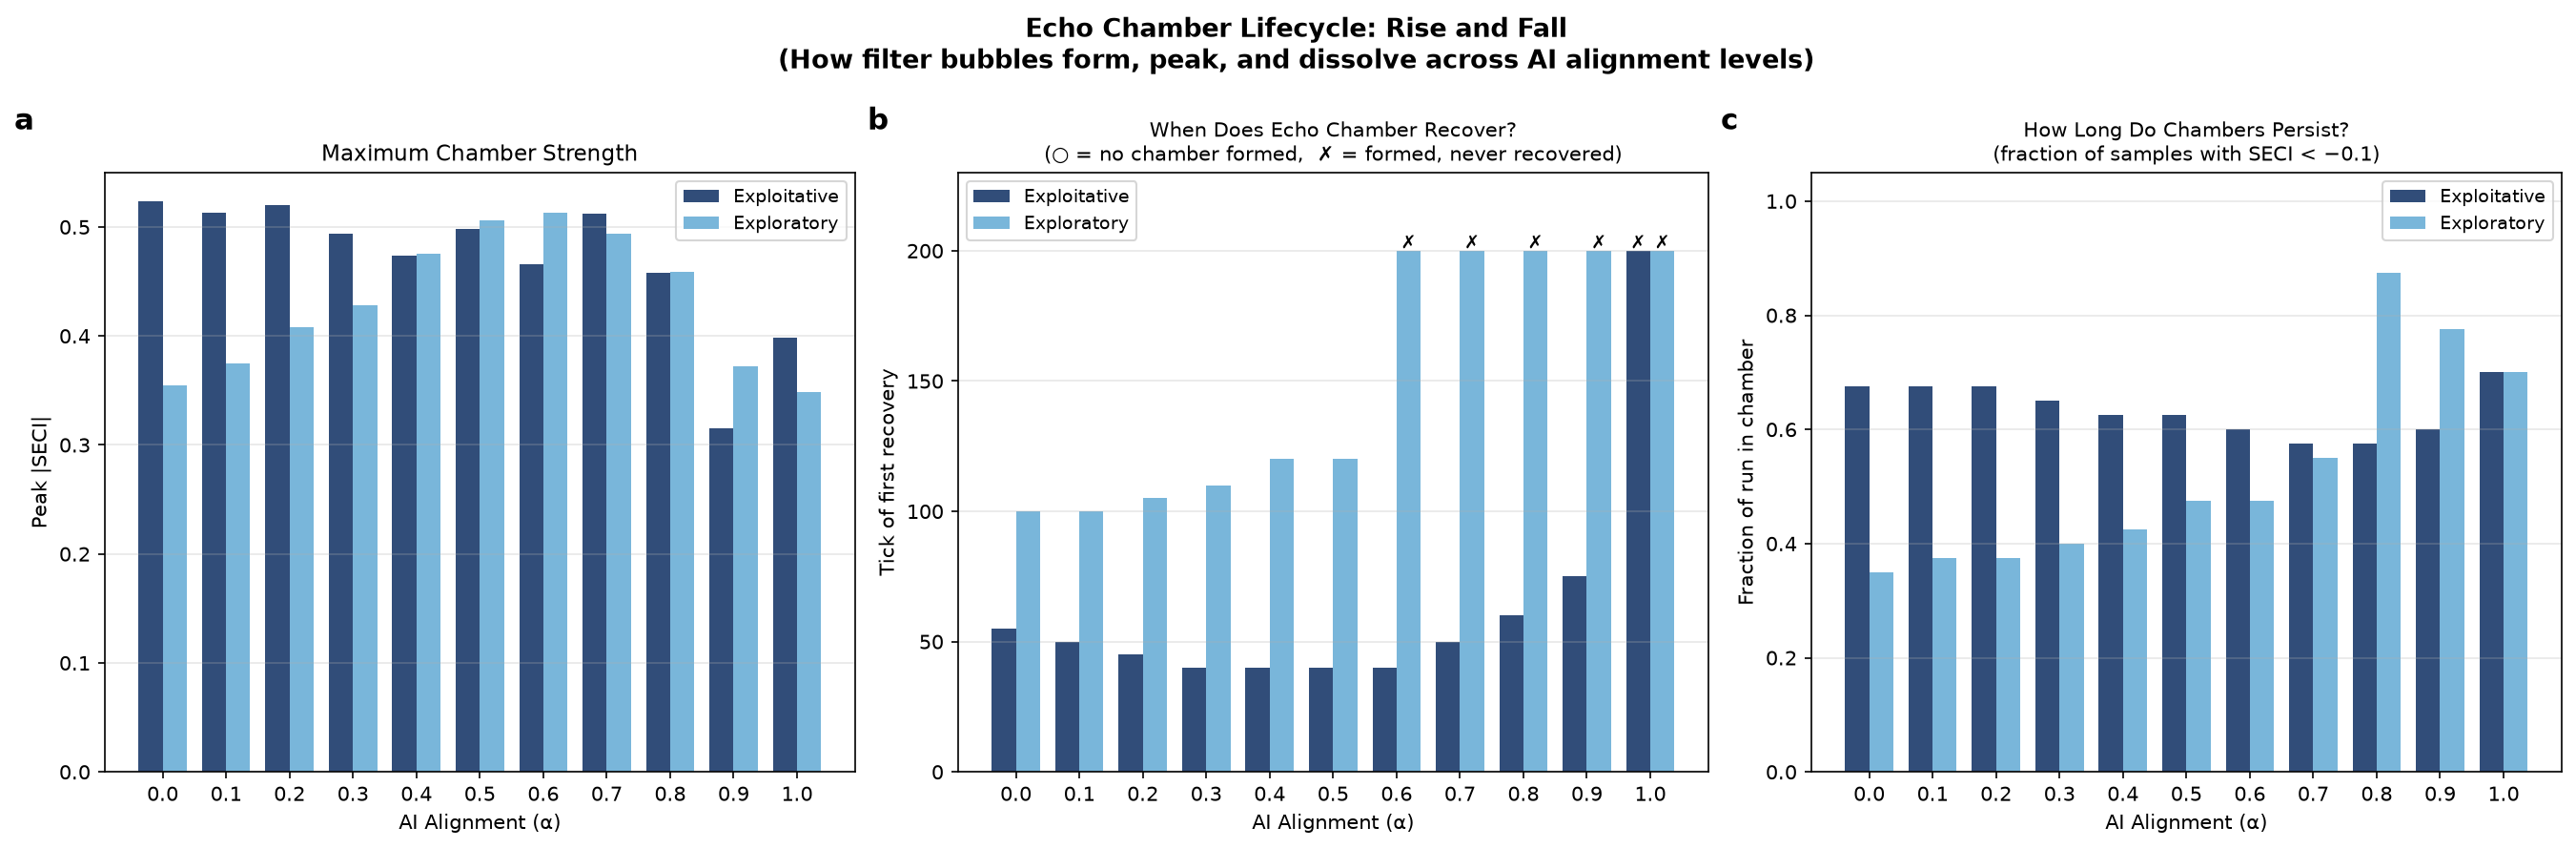
\includegraphics[width=0.95\textwidth]{figS1_lifecycle.png}
\caption{\textbf{Echo-chamber lifecycle across alignment levels} (main
model, per agent type; archived plot from
\texttt{results-mechfix/plots-config-switches/}). Peak chamber strength,
time of first recovery, and fraction of the run spent inside a chamber,
by $\alpha$. Recovery of the exploratory communities' chambers is
progressively delayed as alignment grows and fails within the 200-tick
horizon at high $\alpha$, while peak strength varies little---the harm of
alignment is the failure to dissolve, not deeper peaks.}\label{fig:s1}
\end{figure}

\begin{figure}[h!]
\centering
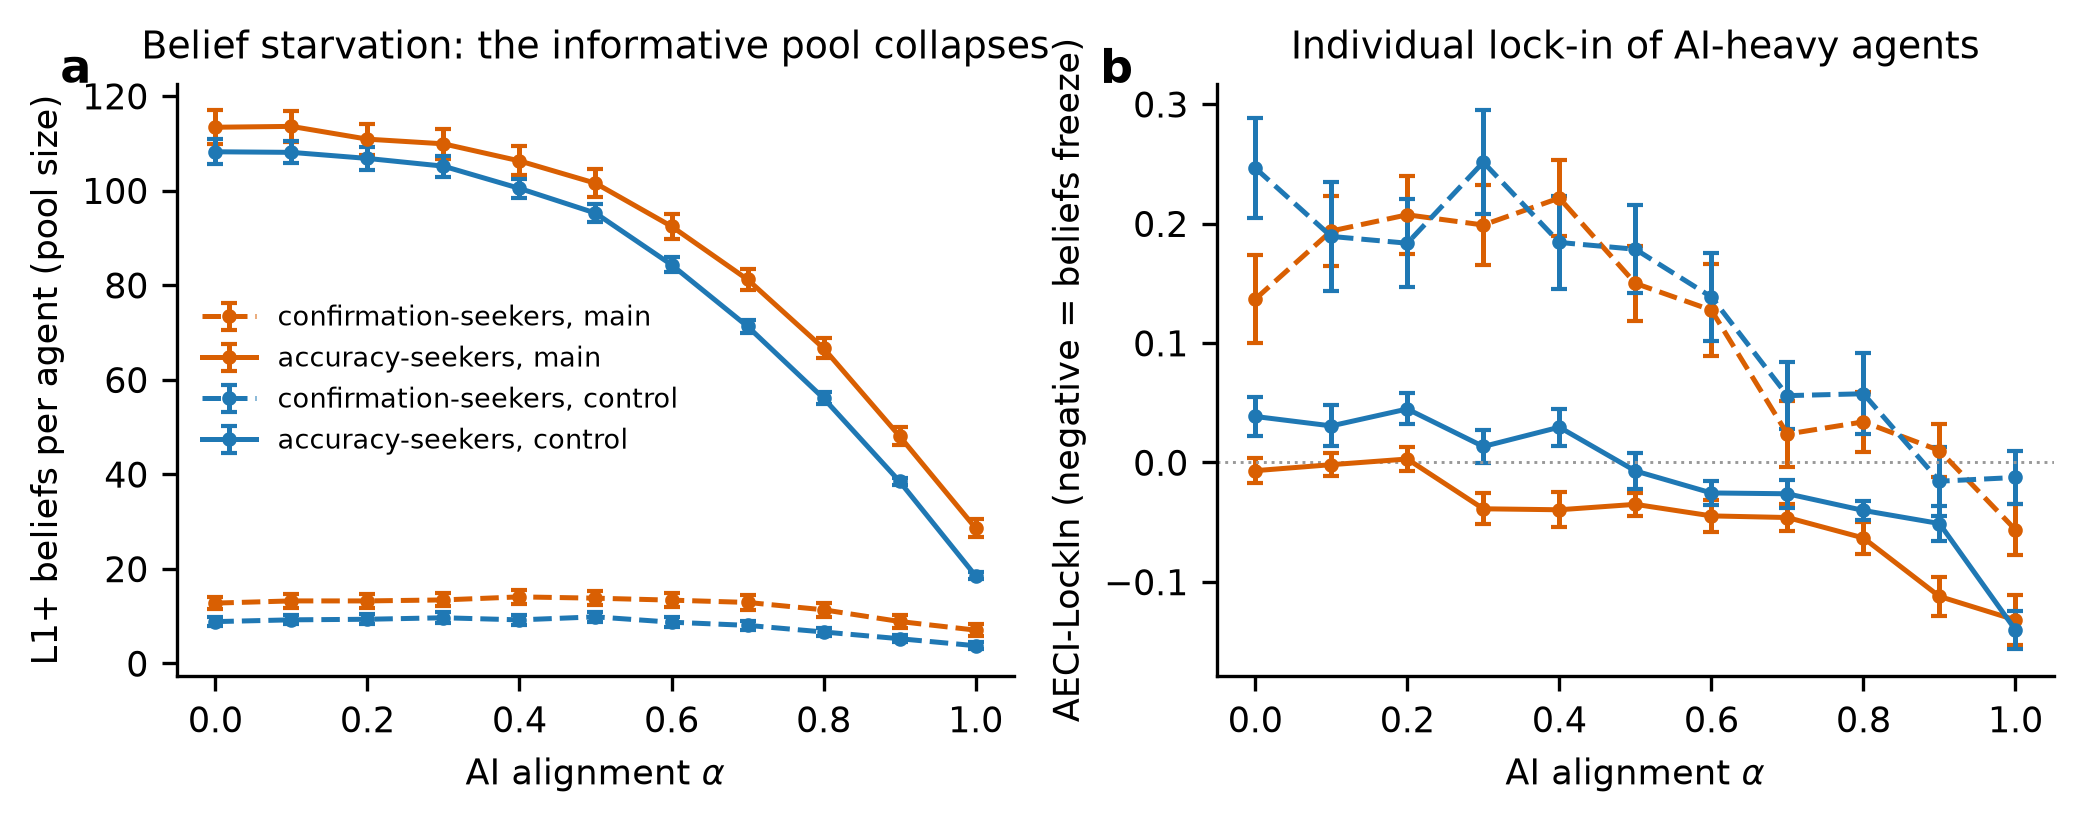
\includegraphics[width=0.95\textwidth]{figS2_starvation.png}
\caption{\textbf{The starvation mechanism.} (\textbf{a}) Informative
(L1+) beliefs per agent against $\alpha$: the accuracy-seekers' pool
collapses from 113 to 29 (main model; 108 to 19 in the control), while
the confirmation-seekers' pool is small at every $\alpha$. (\textbf{b})
AECI-LockIn: the belief revision of AI-heavy accuracy-seekers freezes
with alignment ($-0.01 \to -0.13$); the confirmation-seekers' series
reflects correction churn (Sec.~\ref{si:metrics}). Steady-state means
$\pm$ s.e.m., $N = 20$; orange: main model, blue: control; dashed:
confirmation-seekers, solid: accuracy-seekers.}\label{fig:s2}
\end{figure}

\begin{figure}[h!]
\centering
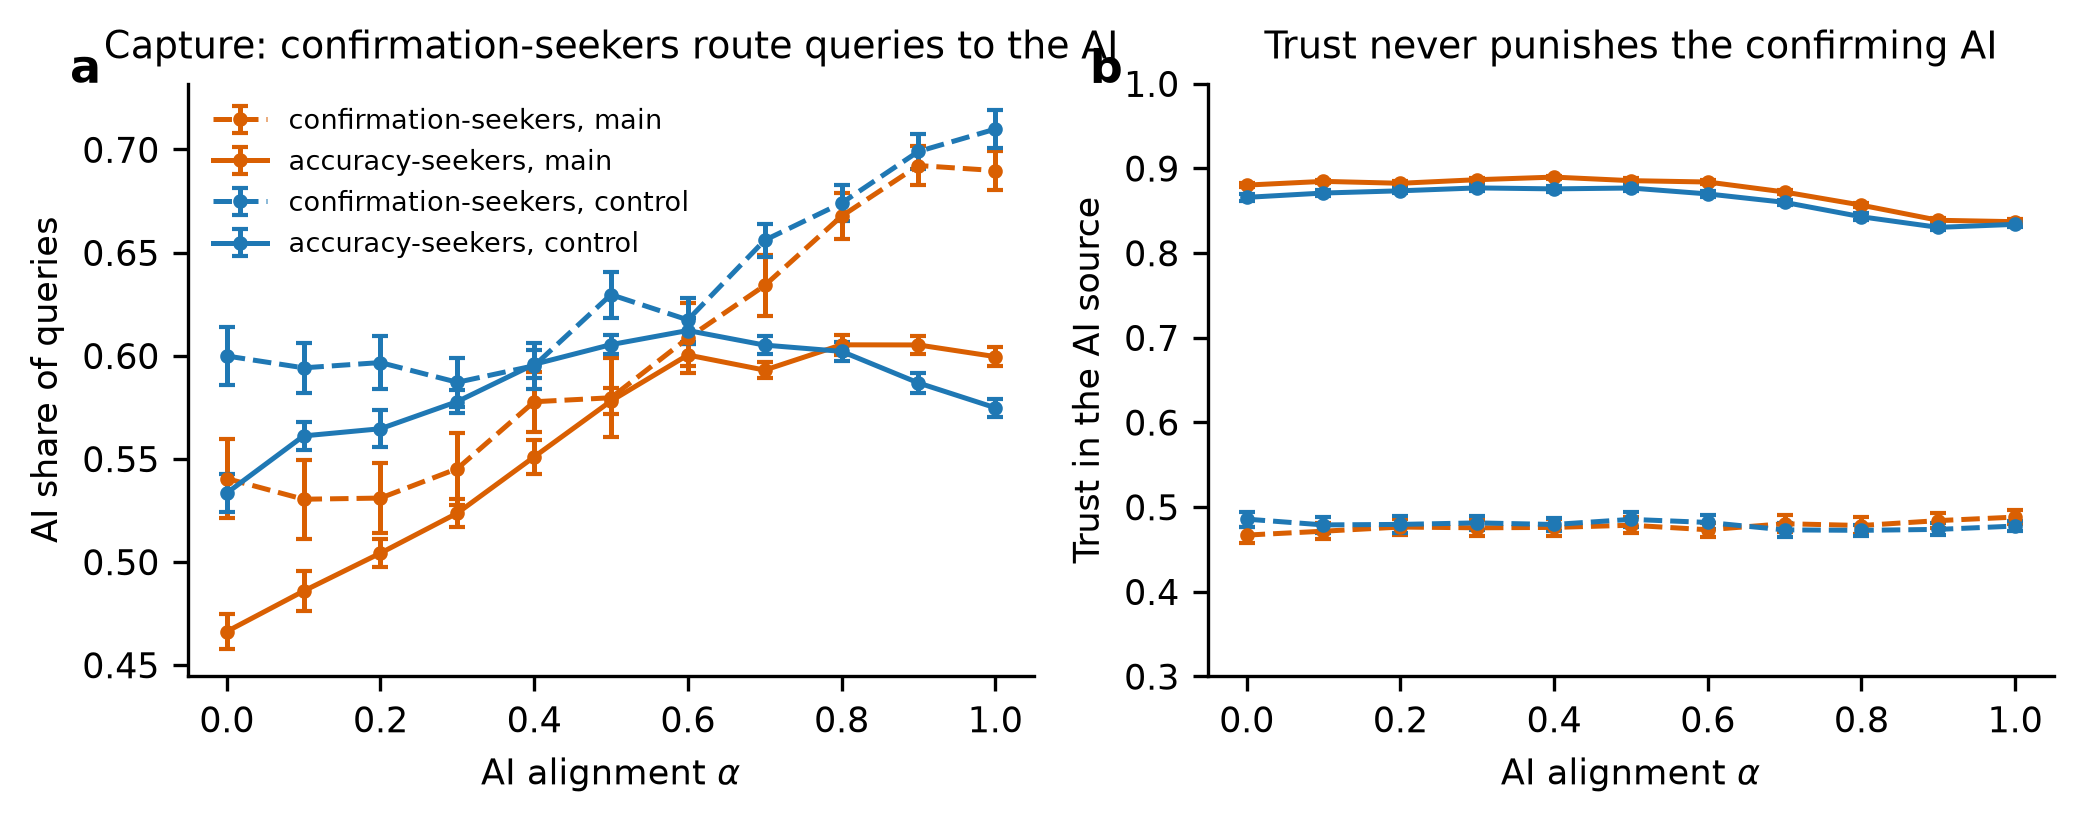
\includegraphics[width=0.95\textwidth]{figS3_feedback.png}
\caption{\textbf{The feedback loop.} (\textbf{a}) AI share of queries per
type: a confirming AI captures the confirmation-seekers (0.54 $\to$ 0.69,
main model) while the accuracy-seekers' share saturates near 0.60 from
mid-alignment. (\textbf{b}) Trust in the AI: the confirmation-seekers'
trust is flat at $\approx 0.47$ at every $\alpha$---capture runs through
the confirmation reward, not trust---and the accuracy-seekers' trust
declines only from 0.88 to 0.84 across the sweep (the base-rate-dominated
verification failure; Table~\ref{tab:s8-salience} for the salience
counterfactual). Conventions as in Fig.~\ref{fig:s2}.}\label{fig:s3}
\end{figure}

\begin{figure}[h!]
\centering
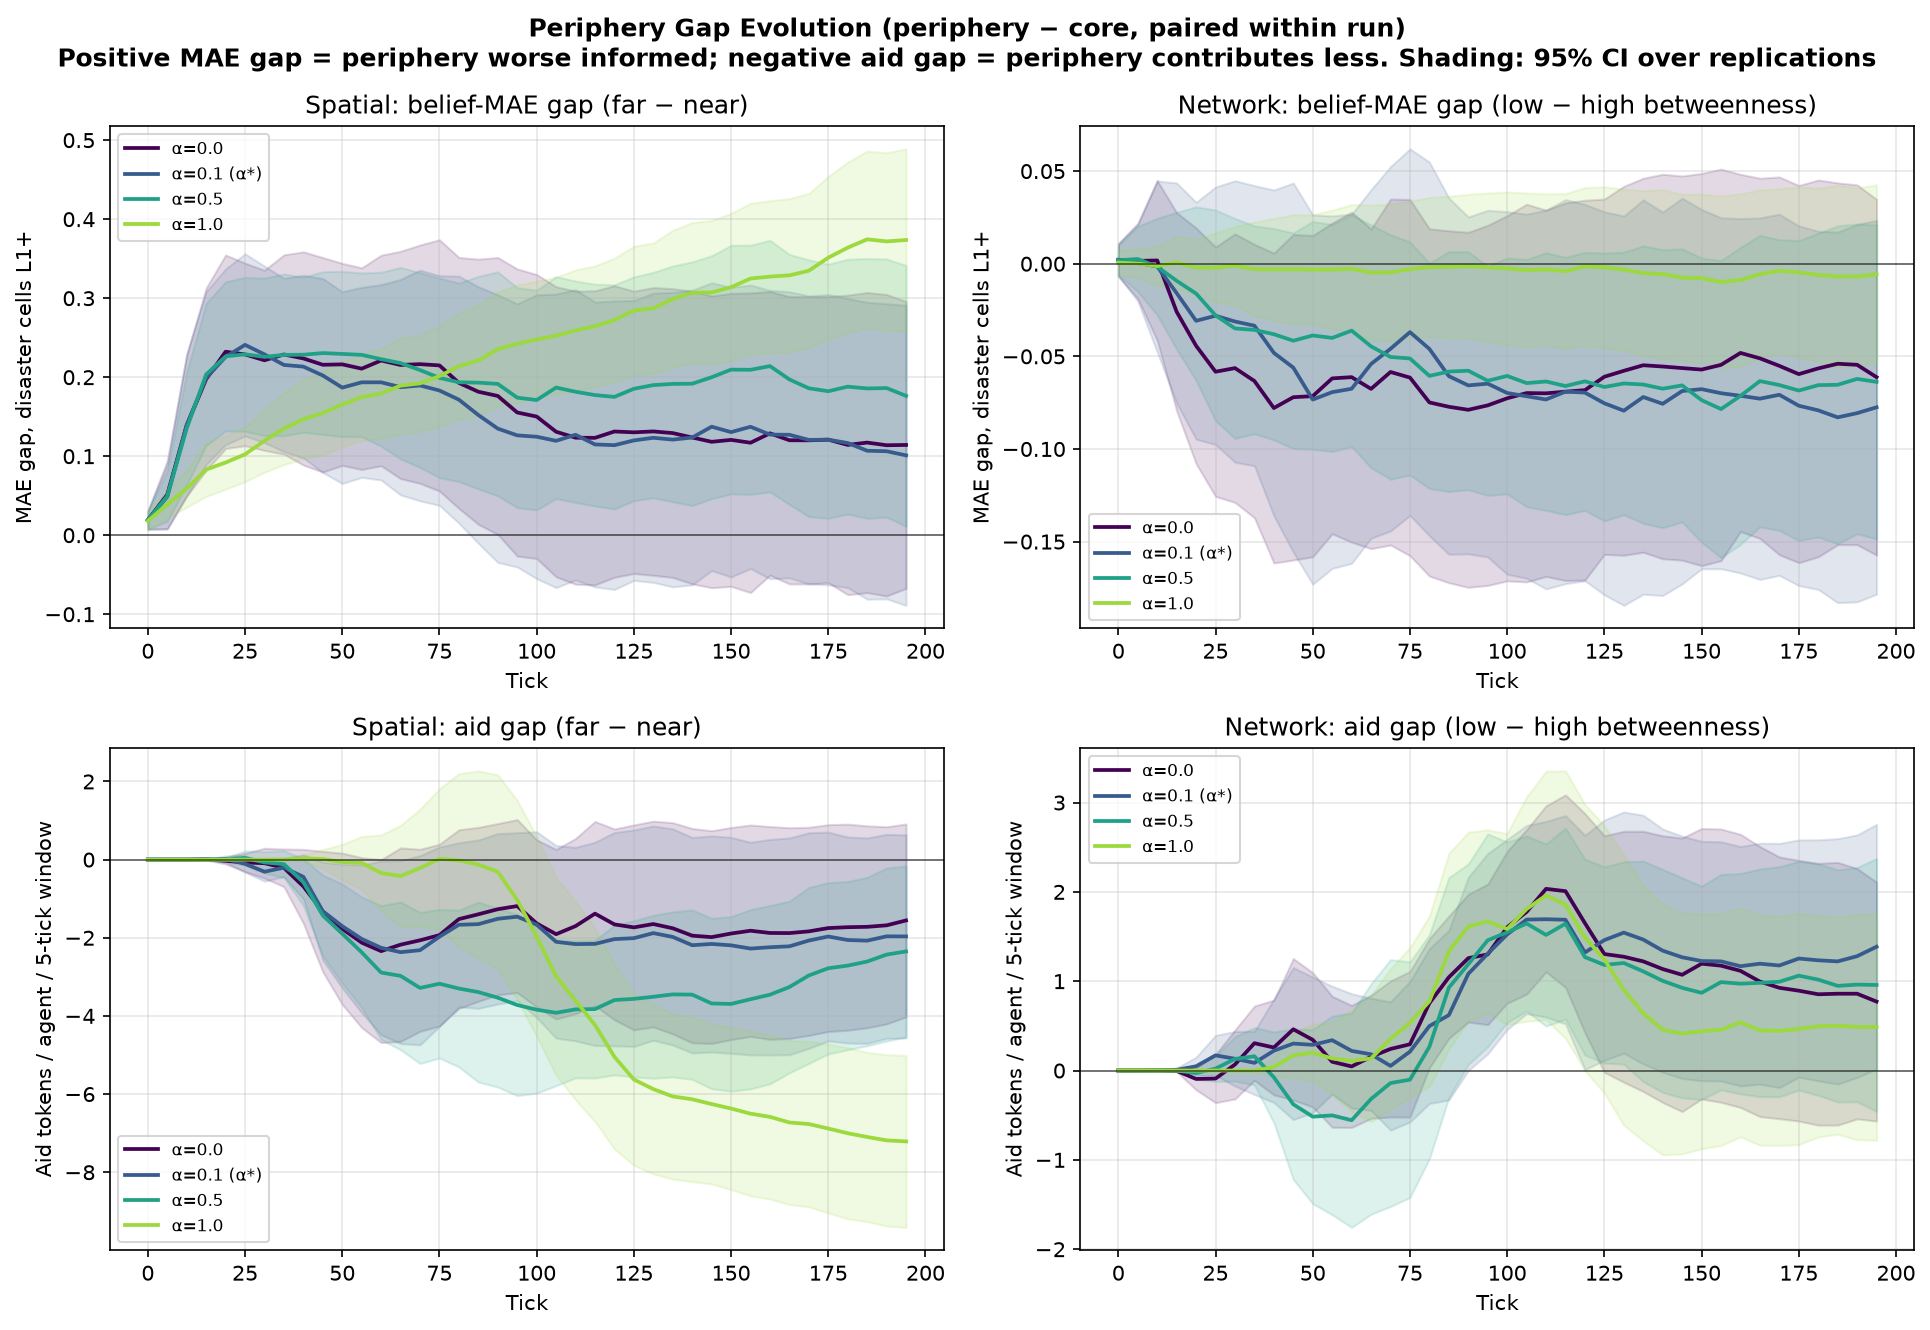
\includegraphics[width=0.95\textwidth]{figS4_periphery_evolution.png}
\caption{\textbf{Within-run evolution of the periphery gaps} (main
model; archived plot from
\texttt{results-mechfix/plots-config-switches/}). Far$-$near belief-error
and aid-contribution gaps over the run at each $\alpha$: the spatial
gradient of Fig.~4 builds gradually and persists through the steady
state rather than arising from initial conditions.}\label{fig:s4}
\end{figure}

\begin{figure}[h!]
\centering
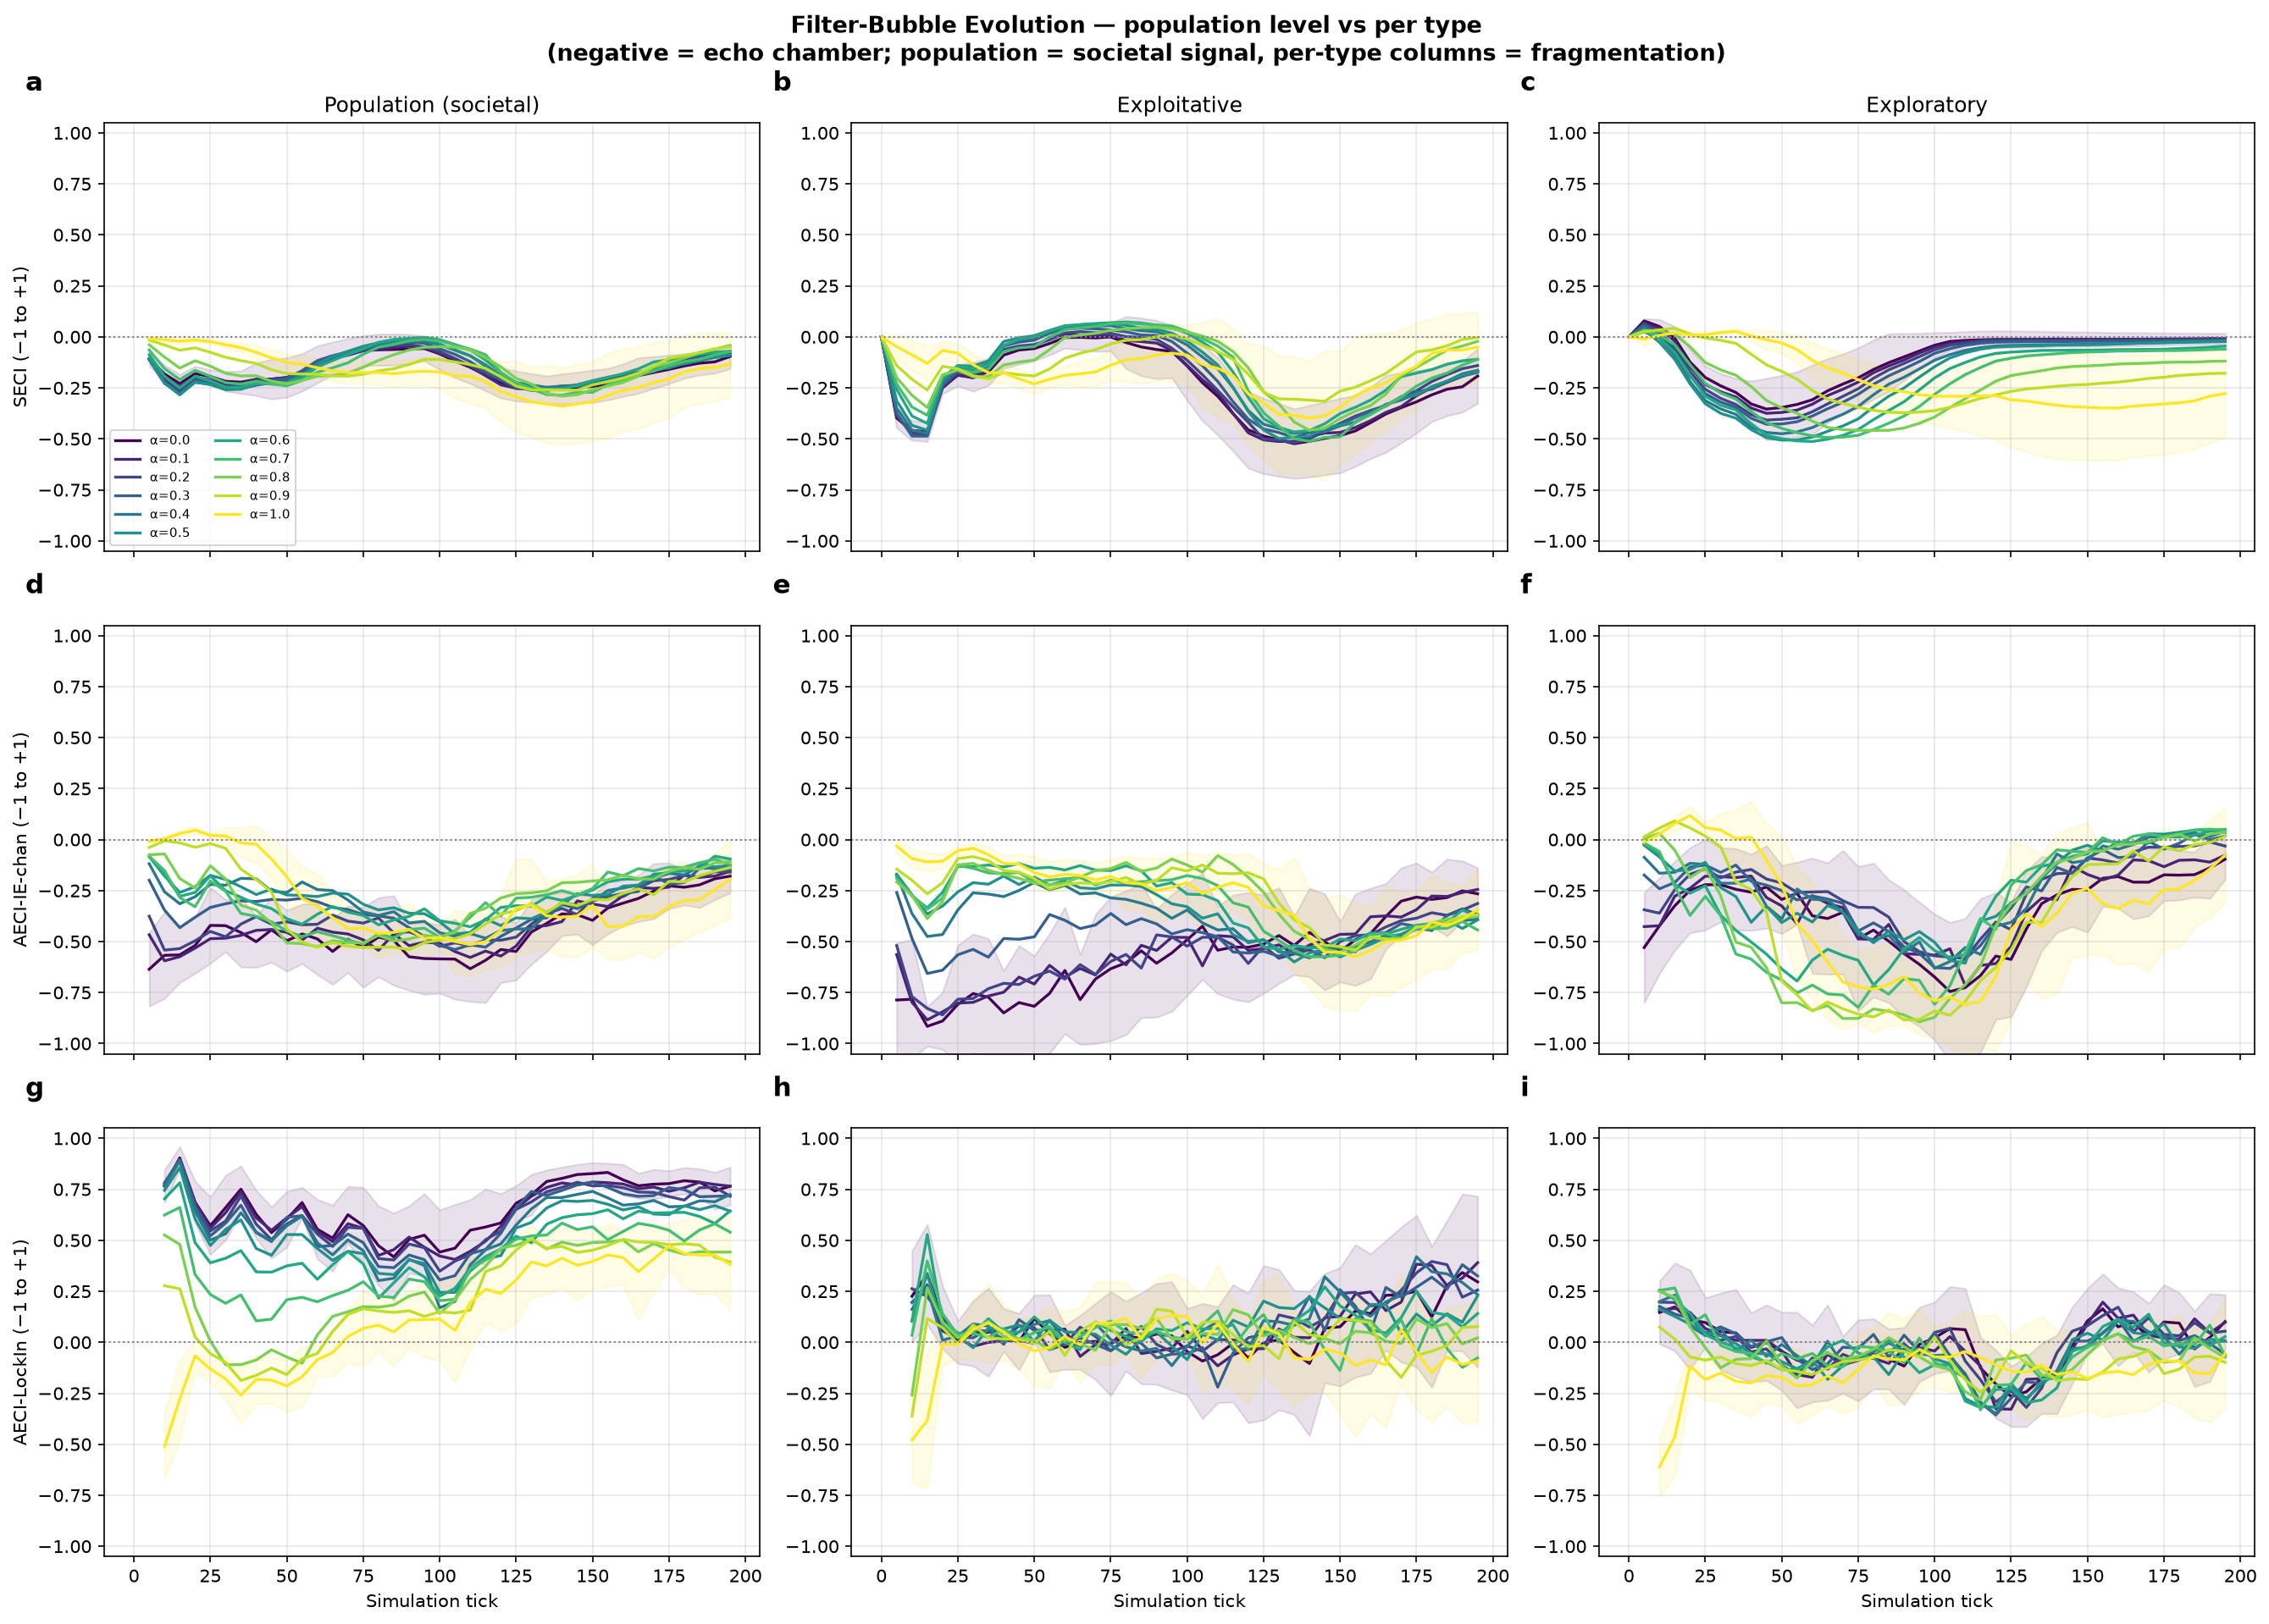
\includegraphics[width=0.95\textwidth]{figS5_population_evolution.png}
\caption{\textbf{Population versus per-type bubble evolution} (main
model; archived plot from
\texttt{results-mechfix/plots-config-switches/}; rows: SECI, AECI-IE,
AECI-LockIn; columns: population, confirmation-seekers,
accuracy-seekers). The population column shows the societal layer: the
served-information index (AECI-IE, population) is U-shaped in $\alpha$
(shallowest near $\alpha = 0.7$), and the population SECI masks the
per-type crossing in which the confirmation-seekers' chamber dissolves
while the accuracy-seekers' deepens.}\label{fig:s5}
\end{figure}

\begin{figure}[h!]
\centering
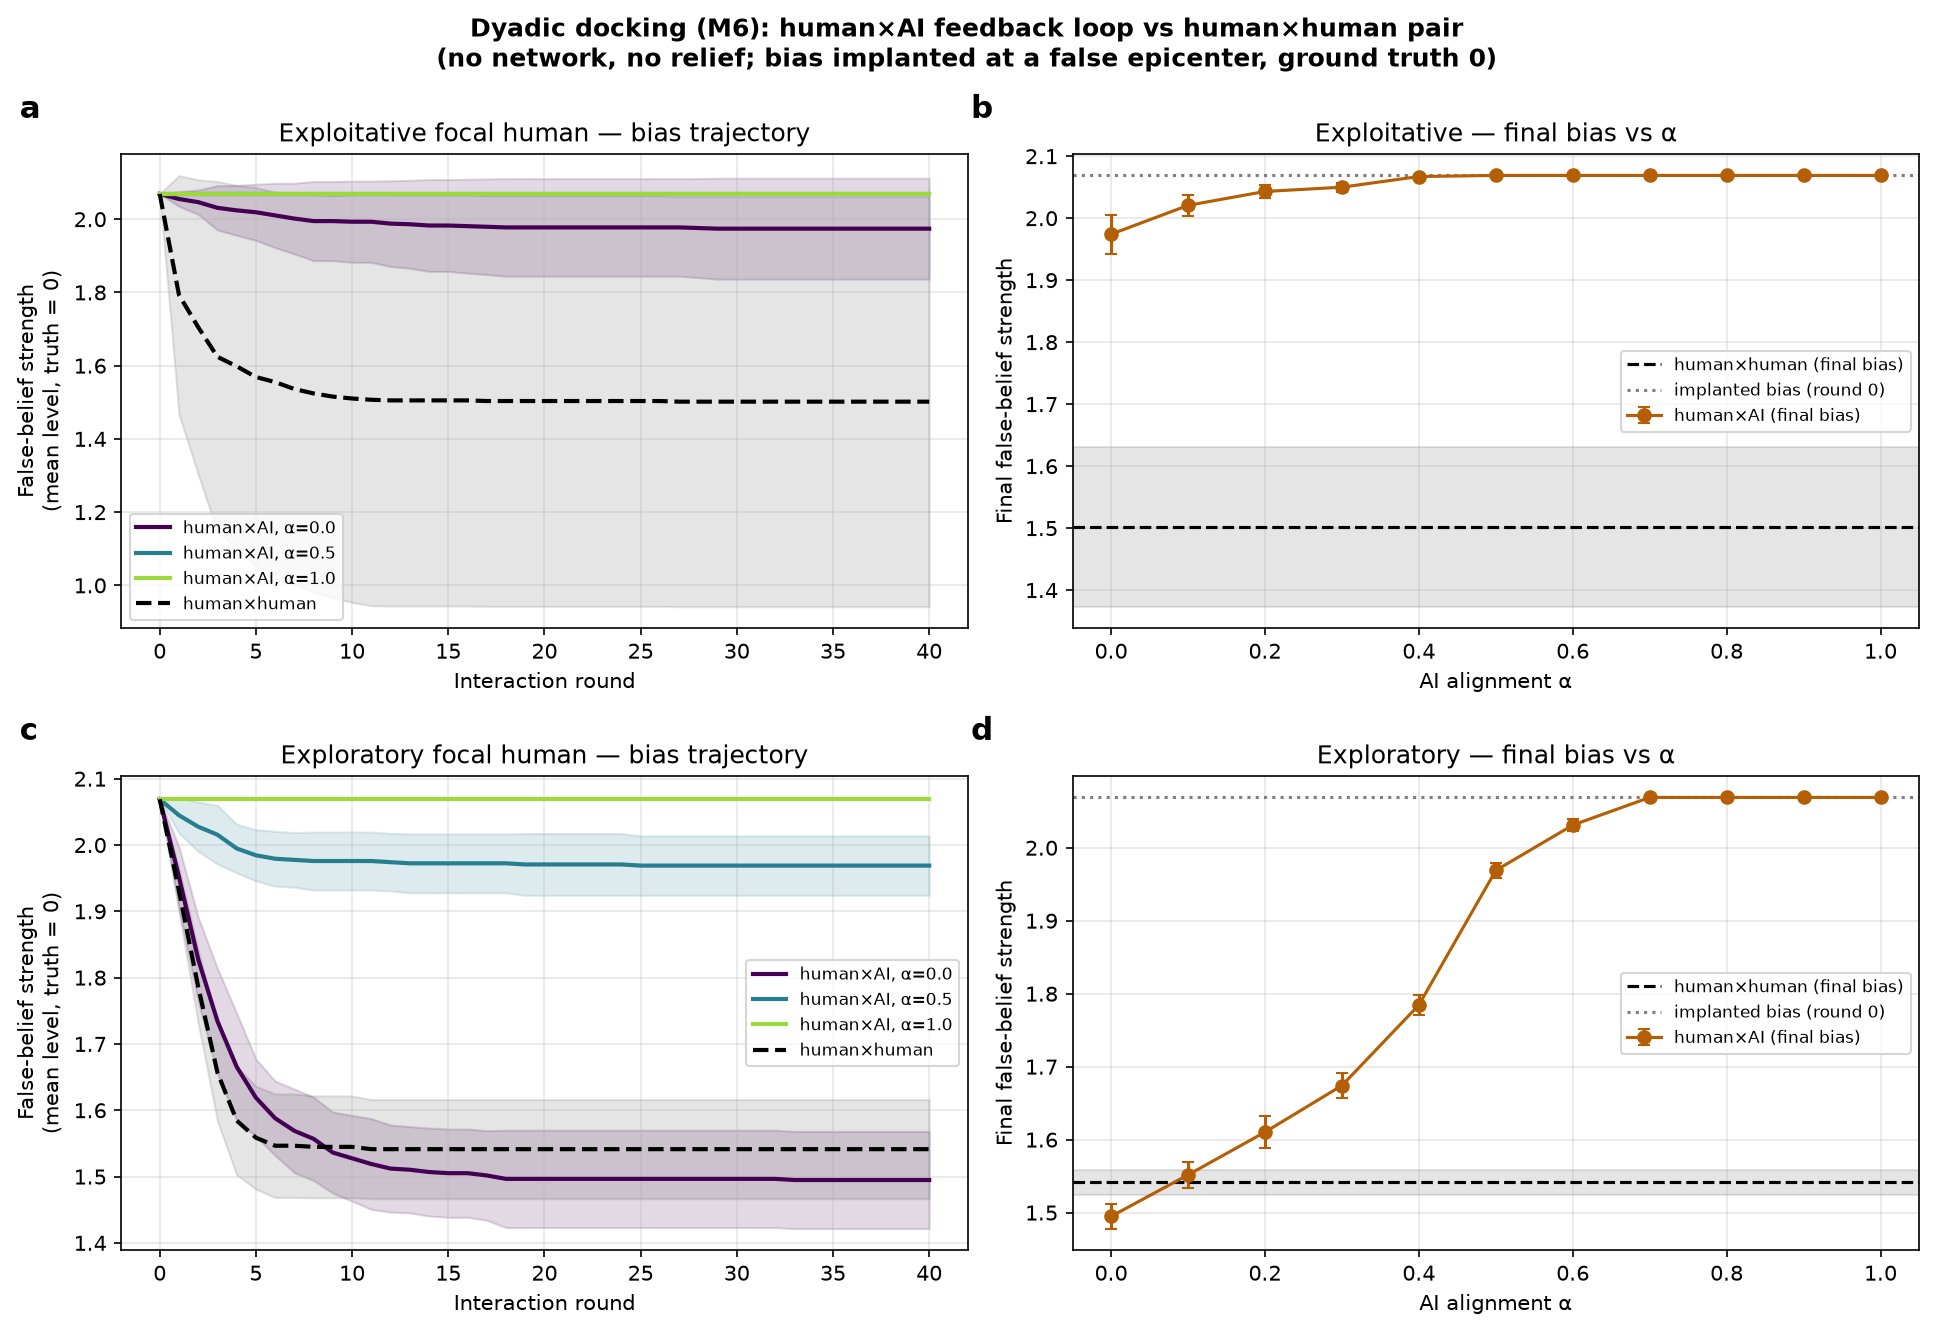
\includegraphics[width=0.8\textwidth]{figS6_dyadic_docking.png}
\caption{\textbf{Dyadic docking against the human--AI feedback-loop
experiments} (archived plot from \texttt{results-docking/}). Final false-belief
level after 40 rounds of one human $\times$ one AI interaction (no
network, no relief feedback), by $\alpha$ and agent type, against a
human--human pair. Bias retention grows smoothly with $\alpha$ and an
aligned AI retains more bias than a human partner---the qualitative
signature of \citet{glickman2024human}.}\label{fig:s6}
\end{figure}

\begin{figure}[h!]
\centering
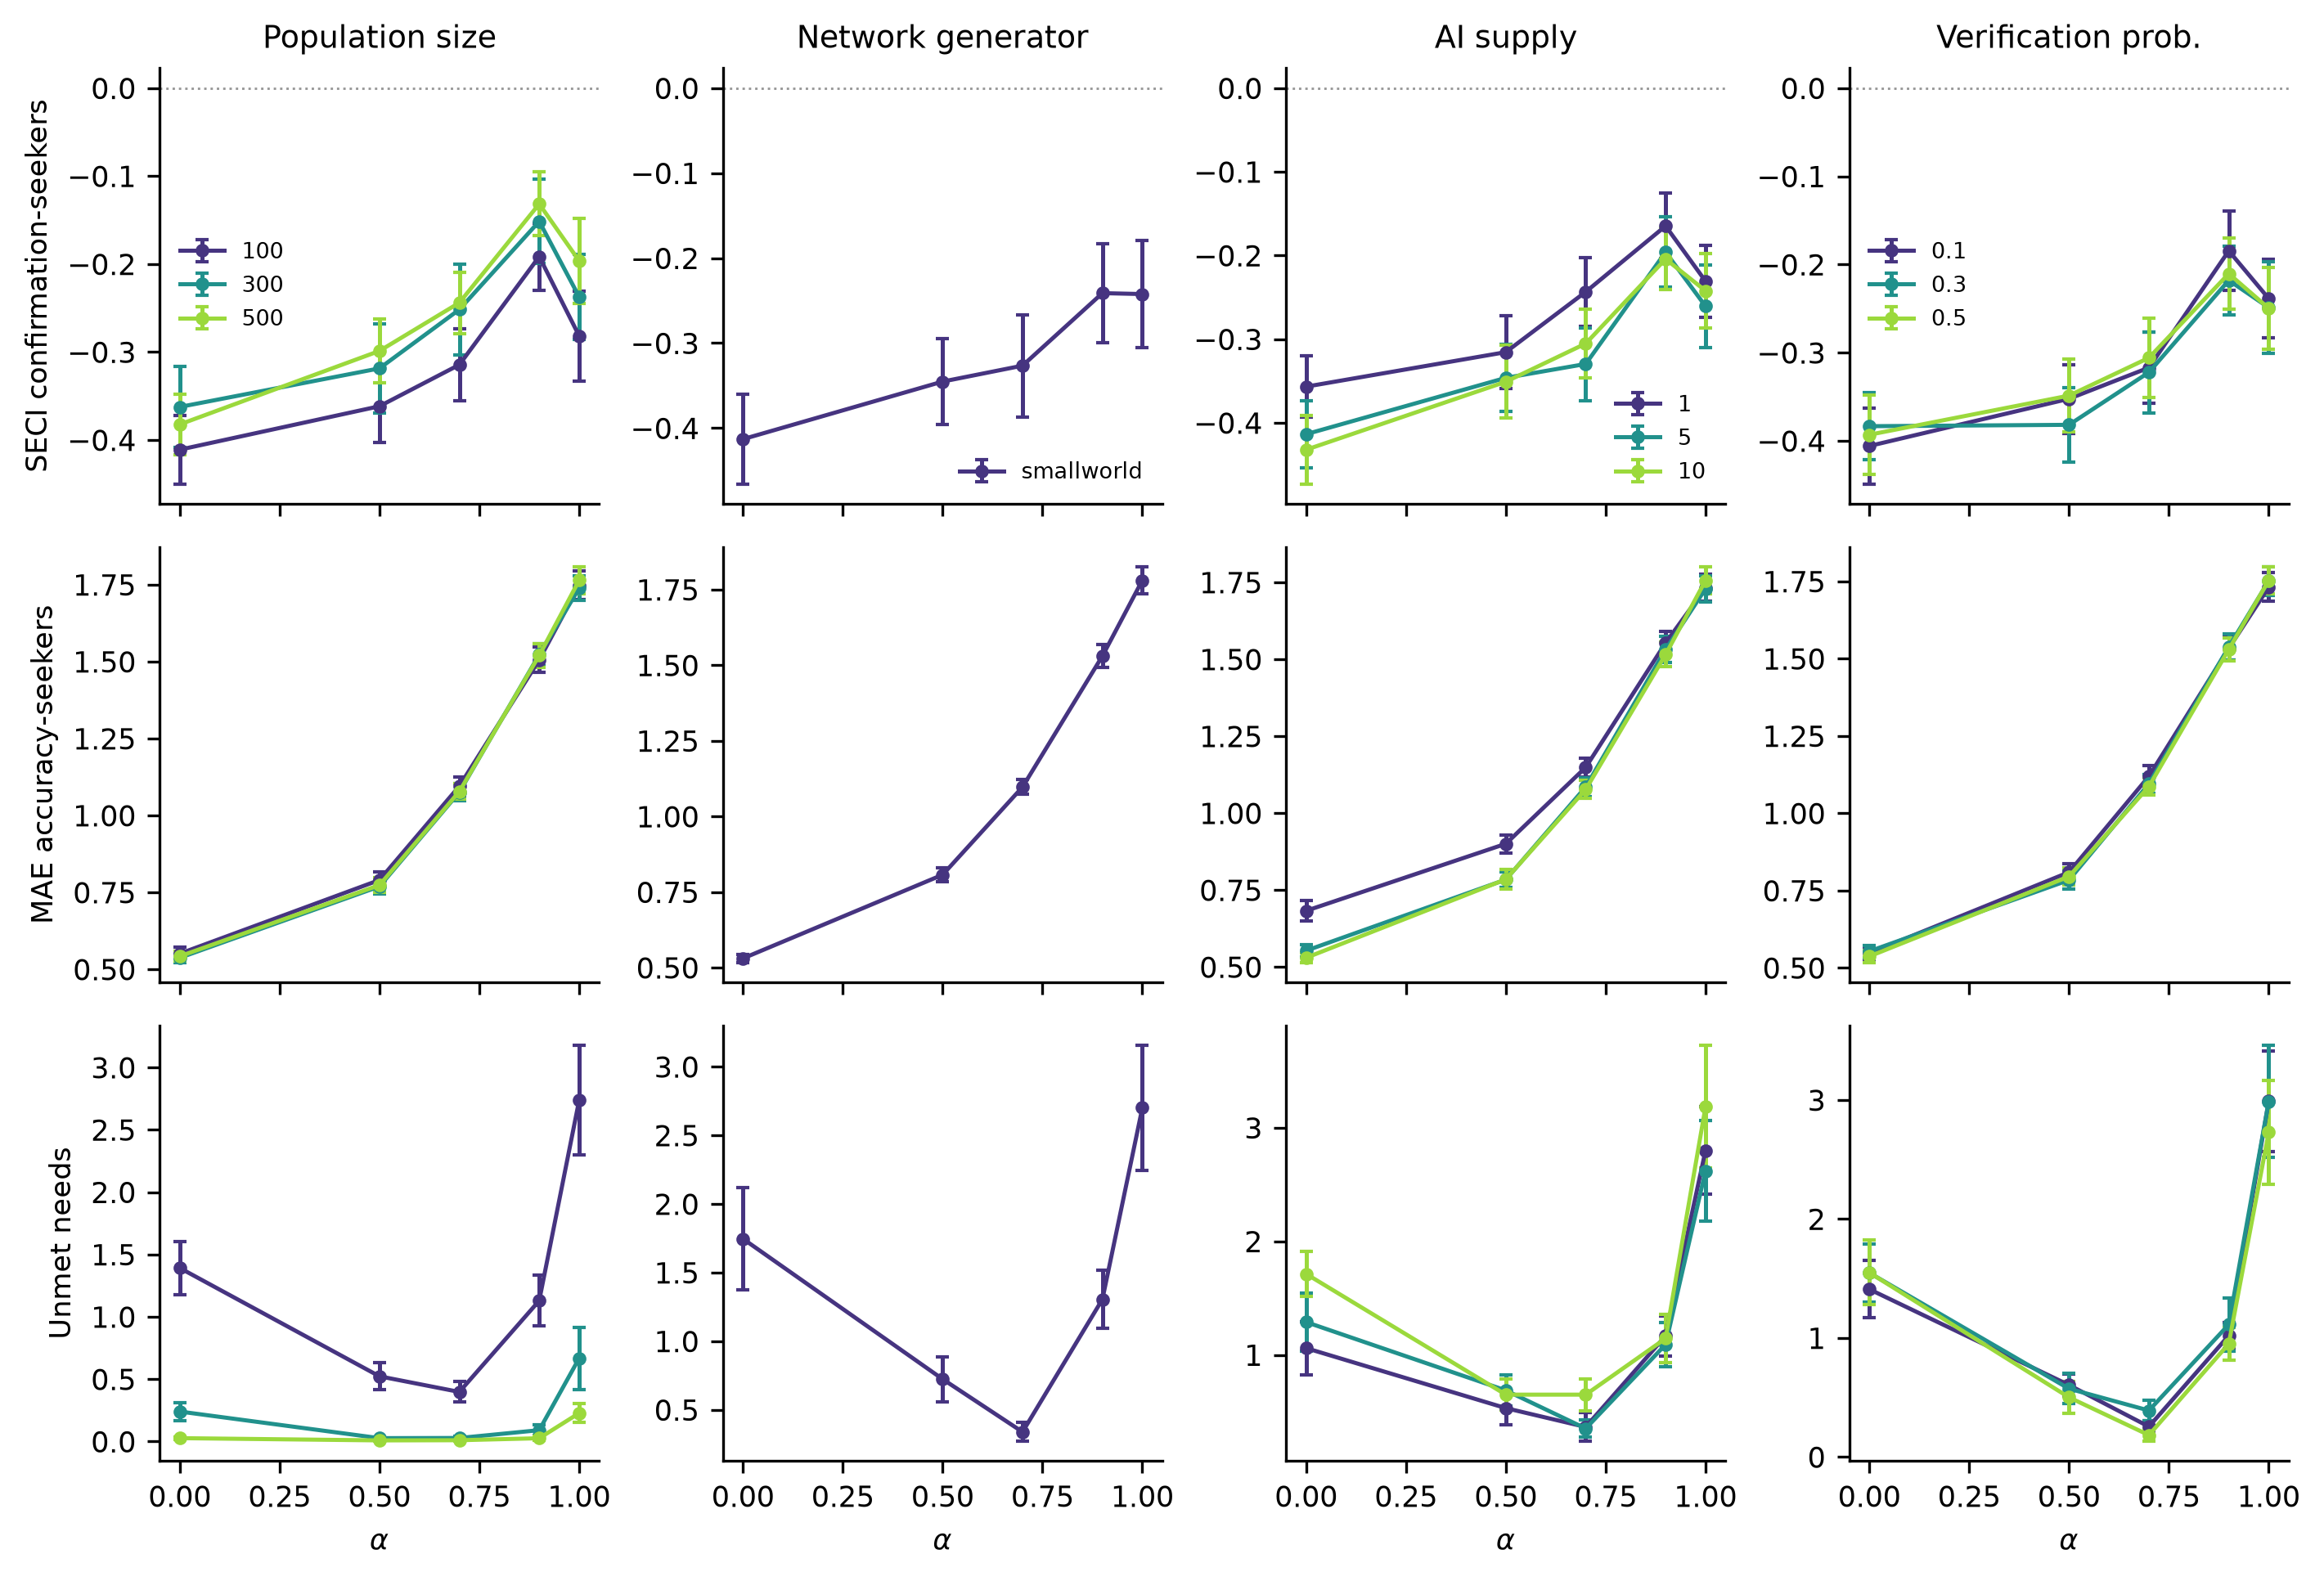
\includegraphics[width=\textwidth]{figS7_robustness.png}
\caption{\textbf{Robustness envelope (M5).} Confirmation-seekers' SECI
(top; the structural-precondition persistence), accuracy-seekers' MAE
(middle; the starvation dose--response), and unmet needs (bottom; the
operational U-shape) against $\alpha$ under perturbations of population
size (100/300/500), within-community network generator (small-world),
AI supply (1/5/10), and verification probability (0.1/0.3/0.5); main
model, $N = 20$, steady-state means $\pm$ s.e.m. All headline mechanisms
hold at every perturbation level.}\label{fig:s7}
\end{figure}

\begin{figure}[h!]
\centering
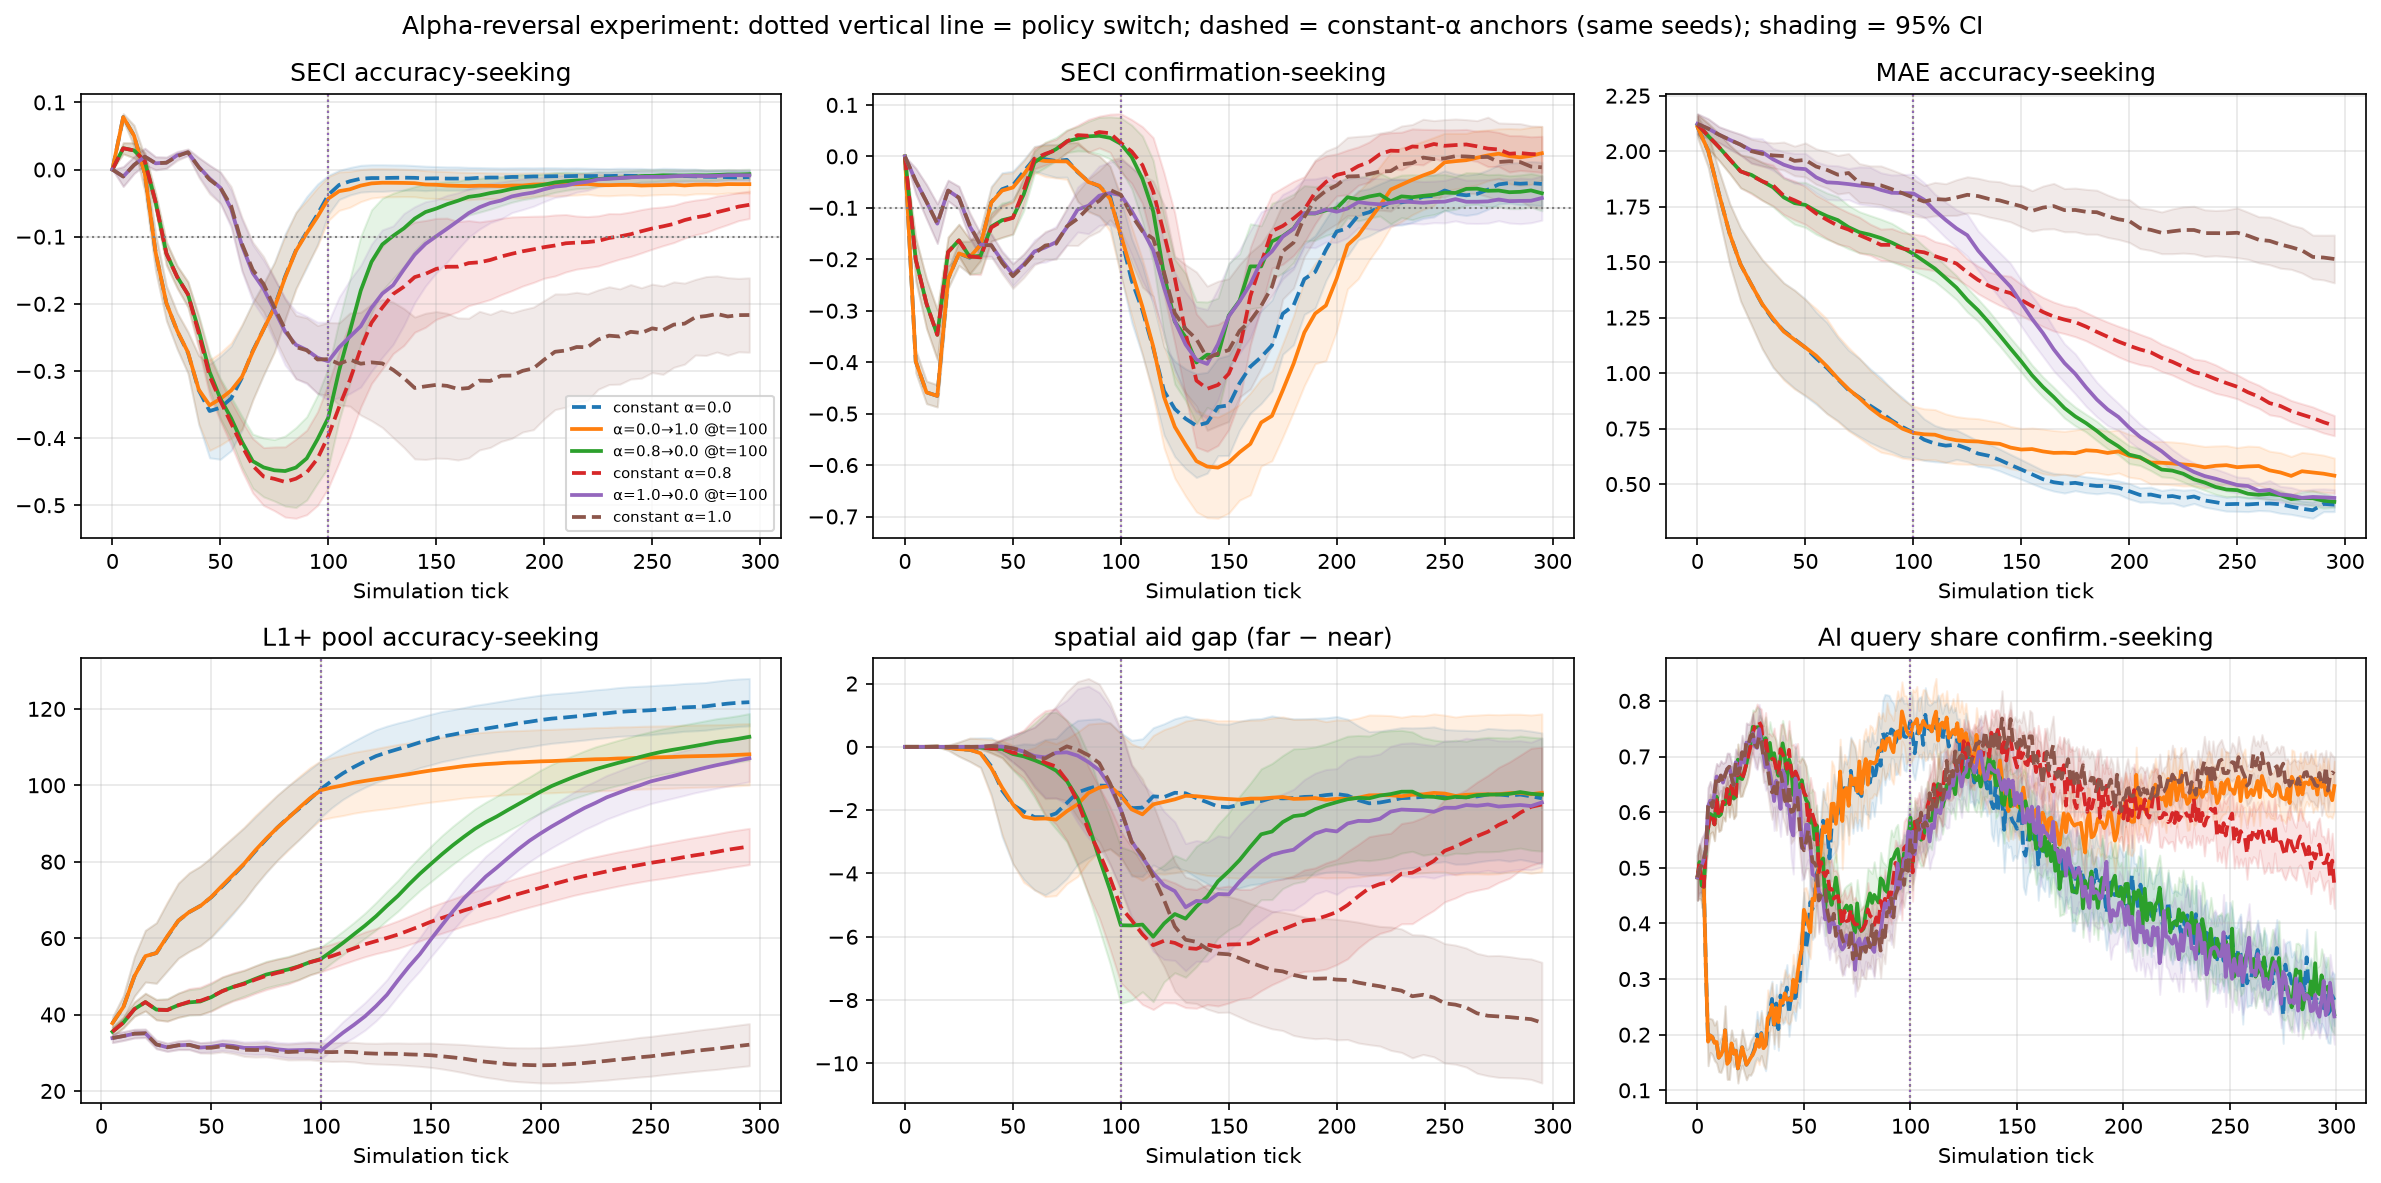
\includegraphics[width=\textwidth]{figS8_reversal.png}
\caption{\textbf{Alignment-reversal (hysteresis) experiment (M9).}
Seed-paired mean trajectories ($\pm$ 95\% CI, $N = 20$) for the repair
switches ($\alpha = 1.0 \to 0.0$ and $0.8 \to 0.0$ at tick 100, dotted
vertical line), the late-onset probe ($0.0 \to 1.0$), and the
constant-$\alpha$ anchors (dashed) on the same seeds; main model, 300
ticks. After the repair, the accuracy-seekers' SECI and the
confirmation-seekers' AI query share return to the truthful-anchor
trajectories (the social layer is a property of the ongoing policy),
while the accuracy-seekers' informative-belief pool and belief error
trail the truthful anchor for the remaining 200 ticks (the epistemic
damage outlives the policy). Under the late-onset switch, the informed
population is buffered: the belief pool stays high and no
accuracy-seekers' chamber re-forms. Statistics in
Table~\ref{tab:s11-lifecycle}.}\label{fig:s8}
\end{figure}

% ============================================================
\clearpage
\section{Supplementary tables}\label{si:tables}

% ---------- Table S1 ----------
\begin{table}[h!]
\centering
\caption{\textbf{Paired per-seed configuration contrasts (main $-$
control) with Holm-corrected significance.} Late-run means; replicate
$i$ shares seed $i$ across configurations. Rows $\alpha \leq 0.7$: $N =
20$ (regression pass, \texttt{results-mechfix/regression/}); rows
$\alpha \geq 0.8$: $N = 50$ (boundary sweep,
\texttt{results-boundary-n50/}). Bold: Holm-adjusted $p < 0.05$ within
outcome. ex = confirmation-seeking (exploitative), er =
accuracy-seeking (exploratory) agents. Full grids for all outcomes in
the named archives.}\label{tab:s1-deltas}
\small
\begin{tabular}{@{}lccccccc@{}}
\toprule
$\alpha$ & $\Delta$SECI$_{\mathrm{ex}}$ & $\Delta$SECI$_{\mathrm{er}}$ & $\Delta$AECI-IE$_{\mathrm{ex}}$ & $\Delta$AECI-IE$_{\mathrm{er}}$ & $\Delta$MAE$_{\mathrm{er}}$ & $\Delta$Unmet & $\Delta$Prec$_{\mathrm{er}}$ \\
\midrule
0.0 & $+0.06$ & $-0.02$ & $-0.03$ & $\mathbf{-0.11}$ & $\mathbf{-0.08}$ & $-0.64$ & $+0.00$ \\
0.3 & $+0.07$ & $-0.02$ & $-0.01$ & $\mathbf{-0.06}$ & $\mathbf{-0.10}$ & $-0.32$ & $+0.00$ \\
0.5 & $+0.01$ & $-0.03$ & $-0.05$ & $\mathbf{-0.05}$ & $\mathbf{-0.16}$ & $+0.06$ & $+0.00$ \\
0.6 & $+0.05$ & $-0.05$ & $-0.03$ & $-0.04$ & $\mathbf{-0.20}$ & $-0.24$ & $+0.00$ \\
0.7 & $-0.10$ & $-0.04$ & $-0.10$ & $+0.03$ & $\mathbf{-0.22}$ & $-0.34$ & $\mathbf{+0.02}$ \\
\midrule
0.8 & $\mathbf{-0.12}$ & $\mathbf{-0.08}$ & $\mathbf{-0.14}$ & $+0.00$ & $\mathbf{-0.19}$ & $\mathbf{-0.78}$ & $\mathbf{+0.07}$ \\
0.9 & $\mathbf{-0.17}$ & $\mathbf{-0.10}$ & $\mathbf{-0.19}$ & $+0.03$ & $\mathbf{-0.17}$ & $\mathbf{-2.21}$ & $\mathbf{+0.14}$ \\
1.0 & $\mathbf{-0.27}$ & $-0.05$ & $\mathbf{-0.34}$ & $\mathbf{+0.23}$ & $\mathbf{-0.18}$ & $\mathbf{-6.56}$ & $\mathbf{+0.33}$ \\
\bottomrule
\end{tabular}

\medskip
\footnotesize
Selected 95\% CIs (boundary rows, $N=50$): $\Delta$SECI$_{\mathrm{ex}}$
at $\alpha=1$: $-0.269$ $[-0.350, -0.189]$ ($p \approx 5\times10^{-8}$);
$\Delta$AECI-IE$_{\mathrm{ex}}$ at $\alpha=1$: $-0.341$
$[-0.404, -0.278]$ ($p \approx 3\times10^{-14}$);
$\Delta$AECI-IE$_{\mathrm{er}}$ at $\alpha=1$: $+0.229$
$[+0.148, +0.310]$ ($p \approx 2\times10^{-6}$); $\Delta$Unmet at
$\alpha=1$: $-6.56$ $[-7.58, -5.54]$ ($p \approx 6\times10^{-17}$);
$\Delta$Prec$_{\mathrm{er}}$ at $\alpha=1$: $+0.33$ $[+0.26, +0.41]$.
AECI-IE columns are the channel-baseline variant
(Sec.~\ref{si:metrics}).
\end{table}

% ---------- Table S2 ----------
\begin{table}[h!]
\centering
\caption{\textbf{$\alpha^{*}$ sensitivity across all 12 composite
definitions, and single-mechanism attribution.} Each configuration's own
within-sweep argmin (locations, not composite values, are comparable).
Ablation A reverts only the exploiters' confirmation reference to the
legacy own-prior rule; Ablation B reverts only the stochastic report
rounding to deterministic rounding (both: main-model configuration).
The main model places $\alpha^{*} = 0.6$ for 7/12 definitions (spread
[0.1, 0.6]); Ablation A is nearly identical (8/12), while Ablation B
fragments the optimum (4/12; spread [0.2, 0.6])---the dose
linearization, not the confirmation reference, drives the composite-robust
interior optimum. The control's bubble composites are interior at
0.8--0.9; the pre-revision corner solution ($\alpha^{*} = 1.0$) was an
artifact of the near-step delivered dose.}\label{tab:s2-astar}
\small
\begin{tabular}{@{}lcccc@{}}
\toprule
Composite & Control & Main model & Ablation A (own ref.) & Ablation B (det.\ round.) \\
\midrule
SECI + AECI-IE (belief baseline)        & 0.8 & 0.1 & 0.6 & 0.3 \\
SECI + AECI-IE + MAE                     & 0.0 & 0.1 & 0.1 & 0.3 \\
SECI + AECI-IE-chan                      & 0.8 & \textbf{0.6} & 0.6 & 0.6 \\
SECI + AECI-IE-chan + MAE                & 0.8 & \textbf{0.6} & 0.6 & 0.3 \\
SECI-pop + AECI-IE-chan-pop              & 0.9 & \textbf{0.6} & 0.6 & 0.6 \\
SECI-pop + AECI-IE-chan-pop + MAE        & 0.8 & \textbf{0.6} & 0.6 & 0.6 \\
SECI + AECI-Var (retired)                & 0.9 & \textbf{0.6} & 0.6 & 0.6 \\
SECI + AECI-Var + MAE (retired)          & 0.8 & \textbf{0.6} & 0.6 & 0.3 \\
SECI only                                & 0.9 & \textbf{0.6} & 0.6 & 0.2 \\
SECI + AECI-Err                          & 0.8 & 0.3 & 0.3 & 0.2 \\
SECI + MAE                               & 0.8 & 0.2 & 0.1 & 0.2 \\
SECI + AECI-Err + MAE                    & 0.7 & 0.3 & 0.3 & 0.2 \\
\bottomrule
\end{tabular}
\end{table}

% ---------- Table S3 ----------
\begin{table}[h!]
\centering
\caption{\textbf{Network-centrality decomposition of alignment harms}
(main model; steady-state means $\pm$ s.e.m., $N = 20$; L1+ belief MAE
and aid tokens sent per agent per five-tick window, by betweenness
quartile). The centrality gaps remain small at every $\alpha$
(network-gap $|\Delta\mathrm{MAE}| \leq 0.07$), in contrast to the
spatial gaps of Fig.~4 (far$-$near MAE gap $+0.12 \to +0.33$; aid gap
$-1.8 \to -6.6$): under mobility, the periphery is spatial, not
graph-positional. In the immobile control all gaps are $\approx 0$ at
every $\alpha$.}\label{tab:s3-centrality}
\small
\begin{tabular}{@{}lcccccc@{}}
\toprule
 & \multicolumn{3}{c}{Belief MAE (L1+)} & \multicolumn{3}{c}{Aid sent per agent} \\
\cmidrule(lr){2-4}\cmidrule(lr){5-7}
$\alpha$ & 0.0 & 0.5 & 1.0 & 0.0 & 0.5 & 1.0 \\
\midrule
Low betweenness (Q1)  & $1.10 \pm 0.04$ & $1.21 \pm 0.04$ & $1.81 \pm 0.04$ & $18.2 \pm 0.5$ & $16.8 \pm 0.5$ & $9.0 \pm 0.7$ \\
High betweenness (Q4) & $1.16 \pm 0.03$ & $1.28 \pm 0.04$ & $1.82 \pm 0.04$ & $17.1 \pm 0.5$ & $15.8 \pm 0.6$ & $8.5 \pm 0.6$ \\
\midrule
Near quartile (spatial) & $1.09 \pm 0.07$ & $1.16 \pm 0.06$ & $1.61 \pm 0.05$ & $18.4 \pm 0.9$ & $17.5 \pm 0.9$ & $12.8 \pm 1.0$ \\
Far quartile (spatial)  & $1.21 \pm 0.06$ & $1.36 \pm 0.04$ & $1.94 \pm 0.02$ & $16.6 \pm 0.9$ & $14.4 \pm 0.7$ & $6.3 \pm 0.5$ \\
\bottomrule
\end{tabular}
\end{table}

% ---------- Table S4 ----------
\begin{table}[h!]
\centering
\caption{\textbf{AI-side confirmation-target ablation (consensus vs.\
individual): verdict.} Seed-paired per-$\alpha$ deltas (consensus $-$
individual, last 75 ticks, both configurations; archive
\texttt{results-ablation-consensus/}, full delta tables in its
\texttt{config-comparison/}).}\label{tab:s4-consensus}
\small
\begin{tabular}{@{}p{4.2cm}p{9.6cm}@{}}
\toprule
Quantity & Result \\
\midrule
SECI (both types), MAE, AI query share, AI trust, LockIn, L1+ pool &
Deltas statistically indistinguishable from zero at every $\alpha$ in
both configurations. \\
Isolated CI exclusions & Scattered, small, consistent with multiple
testing; include the \emph{opposite} sign to chamber amplification
($\Delta$SECI$_{\mathrm{ex}} = +0.09$ at $\alpha = 0.7$, main model). \\
Interior $\alpha^{*}$ & Preserved (consensus [0.2, 0.4] vs.\ individual
[0.3, 0.6]; all interior). \\
\midrule
Verdict & The AI-side targeting rule is behaviorally near-inert: the
trusted-network consensus coincides with the caller's own prior on most
cells. No finding depends on the AI knowing anything beyond the
querier's revealed beliefs. \\
\bottomrule
\end{tabular}
\end{table}

% ---------- Table S5 ----------
\begin{table}[h!]
\centering
\caption{\textbf{Transparency chain: headline quantities across model
revisions} (main-model configuration unless noted). Legacy =
\texttt{results/} (run 32040117179); type-agnostic fix =
\texttt{results-verification/} / \texttt{results-final/} (runs
32298278561 / 32412891328); mechanism revision =
\texttt{results-mechfix/} (run 32821105202, canonical). The qualitative
findings are stable across the chain; the mechanism revision changes the
dose delivery (linear in $\alpha$), which smooths the dose--response and
makes the interior optimum composite-robust.}\label{tab:s5-chain}
\small
\begin{tabular}{@{}lccc@{}}
\toprule
Quantity & Legacy & Type-agnostic fix & Mechanism revision \\
\midrule
Combined SECI, $\alpha{=}0 \to 0.9$ & $-0.23 \to -0.33$ & $-0.21 \to -0.30$ & $-0.20 \to -0.20$ ($-0.28$ at $\alpha{=}1$) \\
Exploratory MAE, $\alpha{=}0 \to 1$ & $0.56 \to 1.72$ & $0.55 \to 1.75$ & $0.54 \to 1.74$ \\
Exploiter AI share, $\alpha{=}0 \to 1$ & $0.34 \to 0.60$ & $0.47 \to 0.70$ & $0.54 \to 0.69$ \\
Unmet needs at $\alpha{=}1$ (control / main) & $11.3$ / $3.3$ & $10.3$ / $3.1$ & $10.2$ / $2.9$ \\
Interior $\alpha^{*}$ spread (main) & $[0.1, 0.8]$ & $[0.3, 0.6]$ & $0.6$ for 7/12; spread $[0.1, 0.6]$ \\
Control bubble $\alpha^{*}$ & $1.0$ (corner) & $1.0$ (corner) & $0.8$--$0.9$ (interior) \\
\bottomrule
\end{tabular}
\end{table}

% ---------- Table S6 ----------
\begin{table}[h!]
\centering
\caption{\textbf{Standardized mixed-model coefficients} (M4;
z-scored late-run outcomes $\sim \alpha + \alpha^2 + \mathrm{config} +
\mathrm{interactions}$, replicate seed as grouping factor; $n = 440$ per
outcome; configuration coded 0 = control, 1 = main model; SD units;
$^{*}p<0.05$, $^{**}p<0.01$, $^{***}p<0.001$; OLS rows used
seed-clustered SEs where MixedLM did not converge). Archive:
\texttt{results-mechfix/regression/}.}\label{tab:s6-regression}
\footnotesize
\begin{tabular}{@{}lccccc@{}}
\toprule
Outcome & $\alpha$ & $\alpha^2$ & config & $\alpha \times$ config & $\alpha^2 \times$ config \\
\midrule
SECI (exploit) & $-0.95$ & $+3.12^{***}$ & $+0.20$ & $+1.07$ & $-2.46^{***}$ \\
SECI (explor) & $+2.86^{***}$ & $-4.58^{***}$ & $-0.02$ & $-0.93^{*}$ & $+0.71$ \\
AECI-IE-chan (exploit) & $-2.79^{***}$ & $+3.74^{***}$ & $-0.20$ & $+1.19$ & $-2.29^{**}$ \\
AECI-IE-chan (explor) & $+6.46^{***}$ & $-7.95^{***}$ & $-0.43^{**}$ & $-1.06$ & $+2.67^{***}$ \\
SECI (population) & $-0.70$ & $+2.69^{***}$ & $+0.04$ & $+1.81^{**}$ & $-4.00^{***}$ \\
AECI-IE-chan (population) & $+3.76^{***}$ & $-3.26^{***}$ & $-0.82^{***}$ & $+0.94$ & $-0.97$ \\
MAE (exploit) & $-0.93^{*}$ & $+1.37^{***}$ & $-0.55^{***}$ & $-0.10$ & $+0.29$ \\
MAE (explor) & $+0.09$ & $+2.99^{***}$ & $-0.14^{**}$ & $-0.51^{*}$ & $+0.12$ \\
Unmet needs & $-7.50^{***}$ & $+9.24^{***}$ & $-0.67^{***}$ & $+4.83^{***}$ & $-6.47^{***}$ \\
Precision (exploit) & $+0.19$ & $-0.89$ & $+0.57^{***}$ & $+0.27$ & $-0.28$ \\
Precision (explor) & $+5.31^{***}$ & $-7.96^{***}$ & $+0.26^{***}$ & $-2.79^{***}$ & $+4.17^{***}$ \\
\bottomrule
\end{tabular}
\end{table}

% ---------- Table S7 ----------
\begin{table}[h!]
\centering
\caption{\textbf{Fixed simulation parameters (all experiments) and their
calibration rationale.}}\label{tab:s7-params}
\footnotesize
\begin{tabular}{@{}lll@{}}
\toprule
Parameter & Value & Rationale / source \\
\midrule
Grid & $30 \times 30$, severity 0--5 & Spatial resolution vs.\ tractability \\
Human agents $N$ & 100 & Network effects at trackable scale (robust 100--500, Fig.~\ref{fig:s7}) \\
AI agents & 5 & $\approx$1 per 20 humans (robust 1--10, Fig.~\ref{fig:s7}) \\
AI sensing fraction & 0.15 of grid per tick & Partial, $\alpha$-independent coverage \\
Share of exploitative agents & 0.50 & Balanced mix; profile sweep varies the cognitive axis \\
Shock probability / magnitude & 0.10 per cell-tick / $\pm 2$ & Persistent non-stationarity \\
Simulation length & 200 ticks & Formation, learning, and steady state (last 75 ticks) \\
Initial trust (human / AI) & 0.30 / 0.25 & Low baseline; slight AI skepticism \\
Q-learning rate / $\epsilon$ & 0.10 / 0.30 & Standard values; continued source diversity \\
Trust learning rate (exploit / explor) & 0.015 / 0.030 & Slow trust revision, type-consistent \\
Relief outcome delay & 15--25 ticks & Humanitarian logistics pipeline \\
Verification lag / probability / noise & $\geq 3$ ticks / 0.3 per tick / $\pm 1$ @ 0.2 & Situation-report channel (robust 0.1--0.5) \\
Report expiry & 30 ticks & Unverified reports yield no learning signal \\
Acceptance $D$, $\delta$ (exploit) & 2.0, 3.5 & Confirmation-seeking profile \\
Acceptance $D$, $\delta$ (explor) & 4.0, 1.2 & Accuracy-seeking profile \\
Confirmation reference & network consensus, fallback own prior & Mechanism (ii); ablation-inert \\
Report rounding & stochastic & Delivered dose linear in $\alpha$ \\
Salience weight $s$ & 0 (default); 1 (counterfactual) & Uniform vs.\ severity-weighted evaluation \\
Mobility (main model) & returner--explorer, home radius 3 & Human-mobility dichotomy \citep{pappalardo2015returners} \\
Bridge probability / decay & 0.15 / $(1+d)^{-2}$ & Sparse weak ties \citep{granovetter1973strength} \\
Query scope (main / control) & network (2-hop @ 0.1) / global & The Gap-1 manipulation \\
\bottomrule
\end{tabular}
\end{table}

% ---------- Table S8 ----------
\begin{table}[h!]
\centering
\caption{\textbf{Salience counterfactual (M7): key cells} (main model,
$N = 20$, steady-state means $\pm$ s.e.m.; archive
\texttt{results-salience/}; the full tables including $s = 0.5$,
which is intermediate throughout, are in
\texttt{salience-tables/robustness\_tables.md}). At $s = 1$ the capture
gradient vanishes (AI query share flat at $\approx 0.48$--$0.51$;
exploiter AI trust $\approx 0.42$ throughout; series in the archive) but
confirmation-seekers retrench socially: at $\alpha = 0$ their chamber
deepens ($-0.52$ vs.\ $-0.37$) and their precision falls ($0.43$ vs.\
$0.57$), with MAE unchanged. Accuracy-seekers' AI trust never drops
below $0.82$ even at full salience (C12).}\label{tab:s8-salience}
\small
\begin{tabular}{@{}llccccc@{}}
\toprule
$s$ & $\alpha$ & SECI$_{\mathrm{ex}}$ & Prec$_{\mathrm{ex}}$ & MAE$_{\mathrm{er}}$ & Unmet & AI trust$_{\mathrm{er}}$ \\
\midrule
0 & 0.0 & $-0.37 \pm 0.03$ & $0.57 \pm 0.04$ & $0.56 \pm 0.02$ & $1.59 \pm 0.27$ & $0.88$ \\
0 & 0.7 & $-0.33 \pm 0.05$ & $0.49 \pm 0.05$ & $1.08 \pm 0.03$ & $0.38 \pm 0.10$ & $0.87$ \\
0 & 1.0 & $-0.28 \pm 0.05$ & $0.36 \pm 0.06$ & $1.73 \pm 0.05$ & $3.15 \pm 0.50$ & $0.84$ \\
\midrule
1 & 0.0 & $-0.52 \pm 0.04$ & $0.43 \pm 0.05$ & $0.58 \pm 0.03$ & $1.95 \pm 0.17$ & $0.90$ \\
1 & 0.7 & $-0.23 \pm 0.04$ & $0.45 \pm 0.05$ & $1.25 \pm 0.03$ & $0.35 \pm 0.06$ & $0.86$ \\
1 & 1.0 & $-0.23 \pm 0.05$ & $0.38 \pm 0.06$ & $1.76 \pm 0.05$ & $2.61 \pm 0.46$ & $0.82$ \\
\bottomrule
\end{tabular}
\end{table}

% ---------- Table S9 ----------
\begin{table}[h!]
\centering
\caption{\textbf{Cognitive-profile sweep: acceptance parameters at each
gap-scalar value.} The gap scalar $g$ scales the difference between the
two types around a shared midpoint while preserving
$D_{\mathrm{exploit}} < D_{\mathrm{explor}}$ and
$\delta_{\mathrm{exploit}} > \delta_{\mathrm{explor}}$; at $g = 0$ both
types are cognitively identical (heterogeneity null), at $g = 1$ the
baseline calibration is recovered. A second axis shifts the absolute
acceptance midpoint $d_{\mathrm{mid}} \in \{2.0, 3.0, 4.0\}$ (closed,
baseline, open).}\label{tab:s9-gap}
\begin{tabular}{@{}ccccc@{}}
\toprule
$g$ & $D_{\mathrm{exploit}}$ & $\delta_{\mathrm{exploit}}$ & $D_{\mathrm{explor}}$ & $\delta_{\mathrm{explor}}$ \\
\midrule
0.0 & 3.00 & 2.35 & 3.00 & 2.35 \\
0.5 & 2.50 & 2.93 & 3.50 & 1.78 \\
1.0 & 2.00 & 3.50 & 4.00 & 1.20 \\
1.5 & 1.50 & 4.08 & 4.50 & 0.63 \\
\bottomrule
\end{tabular}
\end{table}

% ---------- Table S10 ----------
\begin{table}[h!]
\centering
\caption{\textbf{AI in crisis information management: promises and
perils} across the mechanisms of the crisis information cycle, the human
behavioral patterns they interact with, and example
applications.}\label{tab:s10-promises}
\footnotesize
\begin{tabular}{@{}p{2.0cm}p{2.6cm}p{2.6cm}p{2.6cm}p{2.8cm}@{}}
\toprule
Mechanism & Promise of AI & Peril of AI & Human behavior & Example application \\
\midrule
Information collection & Real-time large-scale information collection \citep{narmatha2025disaster} & Exclusion of marginalized or digitally invisible groups \citep{coleman2024weaving} & Sensemaking \citep{klein2010rapid} & Crowd sensing \citep{mai2025evaluating}, wildfire monitoring \citep{roy2024multi} \\
Information sharing & Facilitate access to diverse sources \citep{jeon2024hearhere} & Sharing confined to closed social networks & Trust and alignment, over-reliance \citep{manzini2024should} & Chatbots \citep{urbanelli2024ermes} \\
Decision support & Tailored and verified information \citep{zhao2025tailoring}, recommendations, automated decisions & Promoting high alignment \citep{manzini2024should}; (moral) de-skilling \citep{vallor2015moral} & (Group) decisions \citep{comes2024ai}, cognitive biases \citep{paulus2022influence} & Agentic AI \citep{acharya2025agentic}, early warning \citep{reichstein2025early} \\
\bottomrule
\end{tabular}
\end{table}

% ---------- Table S11 ----------
\begin{table}[h!]
\centering
\caption{\textbf{Echo-chamber lifecycle and alignment-reversal
statistics (per-seed; $N = 20$, main model, 300-tick runs of the M9
experiment).} Top: accuracy-seekers' chamber lifecycle and
confirmation-seekers' capture onset under constant policies (mean $\pm$
95\% CI over replications; dissolution thresholds in
Sec.~\ref{si:lifecycle}). A chamber forms in every replication at every
level with similar peak depth; what alignment removes is dissolution.
Bottom: post-switch outcomes of the reversal conditions; endpoint
values are last-75-tick means. Archive:
\texttt{results-reversal/}.}\label{tab:s11-lifecycle}
\footnotesize
\begin{tabular}{@{}lccc@{}}
\toprule
Constant policy & $\alpha = 0.0$ & $\alpha = 0.8$ & $\alpha = 1.0$ \\
\midrule
Chamber formed (seeds) & 20/20 & 20/20 & 20/20 \\
Formation tick & $22 \pm 2$ & $27 \pm 2$ & $67 \pm 7$ \\
Peak depth (SECI) & $-0.38 \pm 0.08$ & $-0.50 \pm 0.05$ & $-0.44 \pm 0.07$ \\
Dissolved by tick 200 (seeds) & 17/20 & 7/20 & 2/20 \\
Dissolved by tick 300 (seeds) & 17/20 & 12/20 & 3/20 \\
Capture onset (tick) & $59 \pm 2$ & $3 \pm 1$ & $2 \pm 1$ \\
\midrule
Reversal condition & $1.0 \to 0.0$ & $0.8 \to 0.0$ & $0.0 \to 1.0$ \\
\midrule
Chamber standing at switch (seeds) & 19/20 & 20/20 & 5/20 \\
Dissolved after switch (seeds)$^{a}$ & 18/19 & 20/20 & 1/5 \\
Endpoint MAE (accuracy-seekers)$^{b}$ & $0.49 \pm 0.03$ & $0.47 \pm 0.02$ & $0.57 \pm 0.09$ \\
Endpoint L1+ pool$^{b}$ & $102 \pm 6$ & $109 \pm 6$ & $107 \pm 8$ \\
Endpoint SECI (accuracy-seekers) & $-0.01 \pm 0.01$ & $-0.01 \pm 0.01$ & $-0.02 \pm 0.01$ \\
\bottomrule
\end{tabular}

\smallskip
\raggedright\footnotesize
$^{a}$ Denominators: seeds whose chamber episode contained the switch
tick. $^{b}$ Constant-anchor references: MAE $0.41 \pm 0.03$
($\alpha = 0.0$) vs.\ $1.59 \pm 0.10$ ($\alpha = 1.0$); L1+ pool $120
\pm 6$ vs.\ $30 \pm 5$.
\end{table}

\clearpage
\bibliographystyle{unsrtnat}
\bibliography{References}

\end{document}
